\documentclass[%
    school=etsisi,%
    type=pfg,%
    degree=61IW,%
    authorsex=m,%
    directorsex=m,%
]{upm-report}

\addbibresource{references.bib}

\title{Planificación nutricional mediante algoritmos evolutivos}
\author{Javier Quesada Pajares}
\director{Cristian Ramírez Atencia}

\abstract{spanish}{
    
    Para el final.
    
    \textbf{Condensado no quiere decir incompleto}. Debe contener la información más destacable. Lo ideal es que ocupe entre media y una cara de un folio A4. Comenzará por el propósito y principales objetivos de la memoria. Luego hablaremos sobre los aspectos más destacables de la metodología empleada, seguido de los resultados obtenidos. Por último se presentarán las conclusiones de forma condensada.
    
    Debe tener un estilo claro y conciso, sin ambigüedades de ningún tipo. Además, al ser un resumen de todo el contenido, ni que decir tiene que deberá ser lo último que elaboraremos, y deberá mantener una absoluta fidelidad con el contenido de la memoria.
}
\keywords{spanish}{Cuatro o cinco; Expresiones clave; Que resuman; Nuestro proyecto o; Investigación}

\abstract{english}{
    This section must contain the summary that we have written before in Spanish, but in English, as well as the keywords.
}
\keywords{english}{Four or five; Key Expressions; Summarising; Our Project or; Research}

\acknowledgements{
    Aquí los agradecimientos que quieras dar. Y si no quieres, borras la entrada \texttt{\textbackslash acknowledgements} de \texttt{report.tex} y ya está.
}

\begin{document}

\newglossaryentry{arco-perdicion}{
        name=Arco de la Perdición,
        description={Arco único que posee poderes destructivos capaz de desatar grandes catástrofes y de traer desgracias a aquellos que se encuentren en su camino}
}
\newglossaryentry{hacha-batalla}{
        name=hacha de batalla,
        description={Herramienta antigua utilizada en combate, caracterizada por su doble función de arma y herramienta}
}
\newglossaryentry{python}{
    name={Python},
    plural={Pythonacos},
    description={El mejor lenguaje de programación}
}
\newacronym[
    longplural={inteligencias artificiales}
    ]{ia}{IA}{inteligencia artificial}
\newacronym[
    longplural={organizaciones no gubernamentales},
    shortplural={ONG}
    ]{ong}{ONG}{organización no gubernamental}
\newacronym[
    description={Proyecto a realizar al final de una titulación de Grado},
    longplural={Proyectos Fin de Grado}
    ]{pfg}{PFG}{Proyecto Fin de Grado}
\newacronym[
    description={Proyecto a realizar al final de una titulación de Máster},
    longplural={Proyectos Fin de Máster}
    ]{pfm}{PFM}{Proyecto Fin de Máster}
\newacronym[
    description={Role-Playing Game. Juego de rol},
    shortplural={RPG}
    ]{rpg}{RPG}{\textit{Role-Playing Game}}
\newacronym[
    description={S.P.E.C.I.A.L es la sigla usada para los atributos de Fuerza (\textbf{S}trenght), Percepción (\textbf{P}erception), Resistencia (\textbf{E}ndurance), Carisma, (\textbf{C}harisma), Inteligencia, (\textbf{I}ntelligence), Agilidad, (\textbf{A}gility), y Suerte (\textbf{L}uck)},
    ]{special}{SPECIAL}{\textit{Strenght, Perception, Endurance, Charisma, Intelligence, Agility \& Luck}}





\chapter{Introducción}
\label{ch:introduccion}

\section{Contexto}
En los últimos años, la \gls{ia} se ha posicionado como una de las herramientas más útiles e interesantes de las que disponemos. El término \textit{<<inteligencia artificial>>} fue acuñado por primera vez por John McCarthy en la Conferencia de Darmouth de 1956~\cite{dartmouth1956}. Años después de que Alan Turing formulase la pregunta sobre si las máquinas podían pensar y plantease el famoso Test de Turing~\cite{turing1950}, varios científicos se reunieron con el objetivo de discutir acerca de la posiblidad de un artefacto de comportarse de manera inteligente. Se llegó a la conclusión de que todo aspecto del aprendizaje se puede describir con tanta precisión que resulte factible construir una máquina que los simule.

La IA se enfoca en crear sistemas que puedan realizar tareas que normalmente requerirían de inteligencia humana. Aunque ha tenido un reciente auge debido a los chatbots o los asistentes personales, presenta una gran cantidad de finalidades. Dentro de los usos que se le dan a la IA destacan la creación y el análisis de productos o la automatización de servicios, además de la optimización de procesos. Esta optimización se enfoca en encontrar la mejor solución posible a un problema dado dentro de un conjunto de opciones factibles. Los algoritmos de optimización y de personalización permiten, por ejemplo, crear aplicaciones que permiten organizar tareas de manera inteligente~\cite{todoist2024} o termostatos que ajustan la calefacción automaticamente~\cite{googlenest2020}.

Este \gls{pfg} se centrará en la resolución de un problema de optimización, la creación de un menú semanal de comidas personalizado que cumpla distintos objetivos, como el número de calorías diarias o la cantidad de macronutrientes ingeridos. Se hará uso de la computación evolutiva que, mediante algoritmos genéticos, diseñará una dieta equilibrada a partir de la selección, cruce y mutación de los distintos alimentos.


\section{Motivación}

La motivación para realizar este proyecto viene dada por el interés creciente en el área de la inteligencia artificial y cómo ha cambiado la manera de plantear los problemas respecto al pasado. En España, el sector TIC (Tecnologías de la Información y la Comunicación) cuenta con más del 40\% de empresas que usan estas herramientas para la automatización de flujos de trabajo, análisis de datos o para la gestión de la cadena de suministro~\cite{ontsi2023}. Buscan mejorar la precisión y la eficiencia a la hora de diseñar soluciones.

No obstante, no solo en sectores tecnológicos se hace uso de la IA. El médico o el alimentario también están incorporándola de manera gradual. Los diagnósticos de imágenes médicas~\cite{philips2024} o la agricultura de precisión~\cite{majeed2024} son cada vez más comunes. También en la nutrición, relacionada con esto ámbitos, estas tecnologías permiten nuevas posibilidades.

\begin{figure}[H]
    \centering
    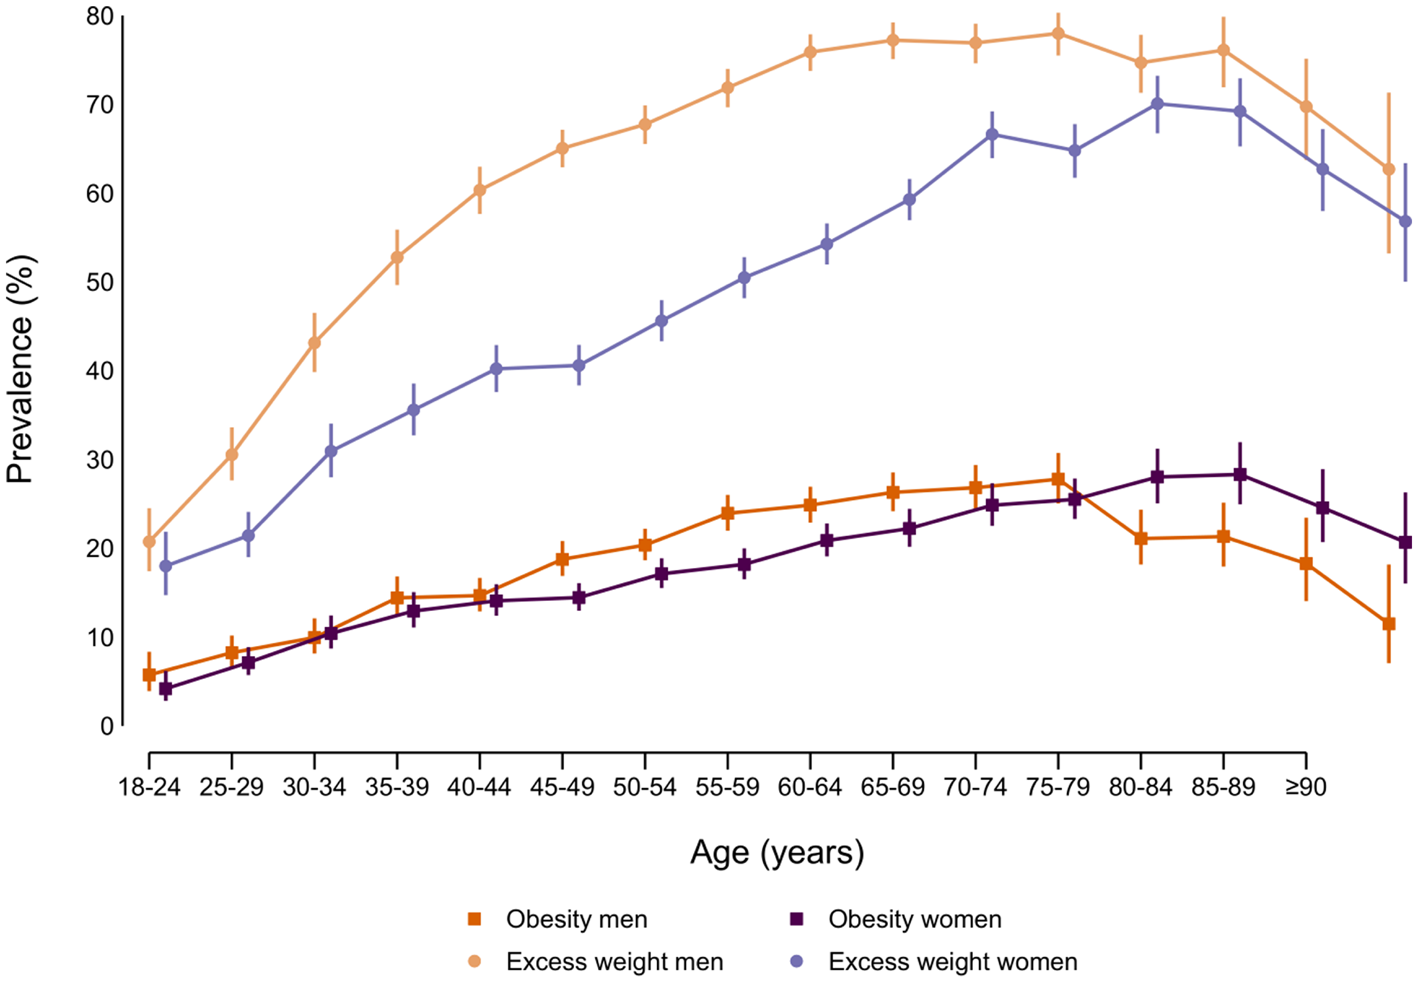
\includegraphics[width=0.75\textwidth]{figures/prevalencia-obesidad.png}
    \caption{Prevalencia (\%) de obesidad y exceso de peso por grupos de sexo y edad. Fuente \cite{ENE-COVID}}
    \label{fig:prevalencia-obesidad}
\end{figure}

Según un estudio llevado a cabo por la Agencia Española de Seguridad Alimentaria y Nutrición (AESAN) y por el Instituto de Salud Carlos III (ISCIII), un 55,8\% de la población adulta española tiene exceso de peso y un 18,7\% padece obesidad, tal y como se muestra en la figura \ref{fig:prevalencia-obesidad}. Esto trae consigo múltiples problemas de salud, como la aparición de enfermedades crónicas o cardiovasculares, complicaciones respiratorias o dificultades al moverse.

Estos datos demuestran la importancia de una buena nutrición y hábitos alimenticios saludables. La planificación nutricional mediante algoritmos genéticos ayuda a comprender cómo se pueden mejorar estos hábitos a través de estas técnicas innovadoras, además de promover una vida sana y bienestar para todos, lo que se relaciona con los Objetivos de Desarrollo Sostenible (ODS)~\cite{ONU2024}, por lo que es un gran aliciente a la hora de realizar este PFG.


\section{Justificación}

En esta sección se deben explicar y argumentar las razones por las cuales se eligió el tema del proyecto, así como su importancia y relevancia. Algunos elementos clave que se pueden abordar en esta sección son:

\begin{enumerate}
    \item \textbf{Relevancia del tema}: ¿Existe alguna necesidad o problema específico que tu proyecto pueda abordar?
    \item \textbf{Justificación teórica}: Mención sobre qué teorías, enfoques o modelos existentes en la literatura respalden la importancia de abordar este tema.
    \item \textbf{Brecha en el conocimiento}: ¿Qué aspectos no se han explorado lo suficiente o no han sido abordados en estudios previos? ¿Cómo puede el proyecto contribuir a cerrar esa brecha en el conocimiento?
    \item \textbf{Contribución práctica}: Aplicaciones del proyecto y cómo pueden beneficiar a la comunidad académica, profesional o a la sociedad en general.
\end{enumerate}

La sección no tiene por qué ser demasiado extensa, ni tiene por qué incluir (o limitarse) a los puntos anteriores, pero debe ser lo suficientemente clara y convincente para que los lectores comprendan por qué el proyecto es relevante y necesario.


\section{Objetivos}

El objetivo general de este proyecto es la creación de un planificación semanal de comidas mediante algoritmos genéticos. Experimentando con diferentes algoritmos se busca crear un menú que cumpla con distintos objetivos nutricionales, como la ingesta calórica diaria, a la vez que limitarse según las restricciones dadas. Los objetivos específicos de este PFG son:

\begin{itemize}
    \item Desarrollar un algoritmo evolutivo capaz de generar menús que cumplan con las restricciones y los objetivos nutricionales establecidos.
    \item Personalizar el algoritmo para la variación de las comidas según las necesidades específicas de los individuos.
    \item Experimentar con distintas configuraciones y variantes del algoritmo genético en busca de encontrar la mejor solución posible.
    \item Evaluar la sensibilidad y eficacia del algoritmo.
    \item Ejecutar pruebas que validen el algoritmo.
    \item Documentar los resultados obtenidos.
\end{itemize}

\begin{comment}
Una de las partes más importante y complicada. Se considera \textbf{la finalidad} del proyecto en cuestión a realizar y suele encajar dentro de una de las siguientes categorías:

\begin{itemize}
    \item \textbf{Contraste} o validación de una hipótesis. Suele usarse en \glspl{pfm}, no tanto en \glspl{pfg}.
    \item \textbf{Desarrollo} o diseño de algo (e.g.~Software, hardware, sistema, edificio). Suele ser el más común en las ingenierías.
    \item \textbf{Estudio} de un tema que deduce o descubre nuevo conocimiento. Suele ser más común en las ramas de las ciencias puras y humanidades.
\end{itemize}

Sirve como primer indicador de la consecución del proyecto, ya que planteando objetivos podemos determinar en las conclusiones su grado de cumplimiento. Ahora bien, ¿cómo determinamos que un objetivo se ha cumplido? pues definiéndolo para que se pueda cumplir, es decir, intentando que sea:

\begin{itemize}
    \item \textbf{Acotado en el tiempo}, así es más fácil establecer un marco temporal para su realización y programar temporalmente las partes de las que se compone.
    \item \textbf{Medible}, para saber cómo de lejos estamos de llegar a un resultado aceptable.
    \item \textbf{Específico}, de manera que esté bien acotado y sea difícil embarcarse en tareas que no nos acerquen a su consecución.
    \item \textbf{Alcanzable}, porque si no lo es, por mucha intención y esfuerzo que le pongamos no se va a terminar.
    \item \textbf{Relevante}, porque si, en un \gls{pfg} para Ingeniería del Software, desarrollamos un producto mecánico para sexar pollos, pues por muy importante que sea, poco tiene que ver con lo que se ha estudiado durante todos estos años.
\end{itemize}

Regla mnemotécnica: \textit{AMEAR}.
\end{comment}

\section{Estructura de la memoria}

En este subapartado se explicará la estructura del documento.

En el capítulo 2, \nameref{ch:estado-arte}, se centra en dar un enfoque general al proyecto. Se da contexto sobre las áreas en las que se basa el proyecto, la inteligencia artificial y los algoritmos evolutivos, además de sobre el tema central del PFG, la planificación nutricional mediante algoritmos evolutivos.

En el capítulo 3, \nameref{ch:marco-teorico}, se aporta la base teórica que en la que se desarrolla el proyecto. Se da una explicación general sobre la inteligencia artificial y se indaga en el algoritmo evolutivo y su funcionamiento.

En el capítulo 4, \nameref{ch:desarrollo}, 
\chapter{Estado del arte}
\label{ch:estado-arte}

\section{Inteligencia artificial}

La inteligencia artificial se puede definir como el estudio y diseño de agentes inteligentes, es decir, de sistemas que perciben su entorno y toman decisiones o acciones que maximizan sus posibilidades de éxito. Este campo se basa en disciplinas como la informática, la lógica o la neurociencia, que contribuyen a la simulación de capacidades cognitivas humanas en máquinas.

Los agentes inteligentes, que son la base de este campo, se clasifican según su capacidad de reconocer y actuar en el entorno. Se pueden encontrar desde agentes simples, que responden directamente a estímulos, hasta agentes basados en utilidad, que evalúan si los resultados de sus acciones son satisfactorios. En estos agentes avanzados, la racionalidad es esencial. Es la habilidad de realizar elecciones óptimas que maximicen la posibilidad de alcanzar objetivos. Utilizando distintas herramientas de lógica, los agentes inteligentes pueden formular y modificar conocimientos, deduciendo nueva información.

El razonamiento lógico también juega un papel fundamental en muchos métodos de inteligencia artificial. Un ejemplo de esto son los algoritmos evolutivos, que se inspiran en los procesos biológicos de la evolución para resolver problemas complejos. Estos algoritmos utilizan principios como la selección natural, el cruce y la mutación para mejorar progresivamente una población de posibles soluciones hacia un objetivo deseado. Al aplicar estos procesos evolutivos, pueden desarrollar soluciones eficientes a problemas que serían difíciles de resolver mediante métodos tradicionales.

El campo de la IA en la actualidad se encuentra en un estado de rápida evolución. Su capacidad para analizar y procesar grandes cantidades de datos o para mejorar la eficiencia en distintas industrias han hecho que se trate de una tecnología en auge. El estudio de \textit{McKinsey \& Company (2022)}~\cite{mckinsey2022ai} estima que el \textit{50\%} de las empresas ya usan IA en sus tareas diarias, donde destacan la optimización de servicios, la creación de productos y el análisis del servicio al cliente.

El informe \textit{''AI Index Report 2024''} (2024)~\cite{aiindex2024} muestra que la IA ya supera a las habilidades humanas en ciertas tareas, como en la clasificación de imágenes, con una precisión del \textit{97\%} respecto al \textit{95\%} de los humanos, o en juegos como el ajedrez, donde supera consistentemente a los jugadores humanos.

\begin{comment}
    Aunque sin duda, el mayor crecimiento en los dos últimos años corresponde a las herramientas relacionadass con la \textit{Inteligencia Artificial Generativa (IAG)}. Esta rama se centra en crear modelos capaces de generar contenido, como conversaciones, imágenes, vídeos o música. Aprende de datos ya existentes y produce nuevos con características similares. En este ámbito destaca la empresa \textit{OpenAI}, que cuenta con \textit{ChatGPT}, capaz de generar texto lógico y actuar como chatbot, o con \textit{Dall-E}, que puede generar imágenes en base a la descripción que se entregue, como la que se muestra en la figura \ref{fig:dall-e}.

    \textit{''The state of AI in 2023: Generative AI's breakout year''} (2023)~\cite{mckinsey2023state} muestra que el \textit{79\%} de los encuestados dice haber tenido al menos alguna exposición a la IAG, lo que indica que es la herramienta de IA que más rápido está captando el interés del público general.

    \begin{figure}[H]
        \centering
        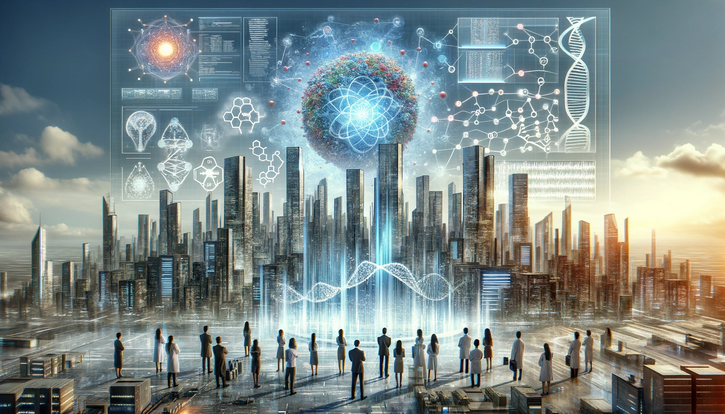
\includegraphics[width=0.5\textwidth]{figures/dall-e.png}
        \caption{Imagen generada con DALL-E 3.}
        \label{fig:dall-e}
    \end{figure}
\end{comment}

Si bien existen diversas formas de clasificar la IA, una de las más interesantes respecto a este PFG es la basada en la representación y el procesamiento del conocimiento. Según esta clasificación, existen dos tipos: la simbólica y la subsimbólica. La IA simbólica utiliza representaciones explícitas y legibles para los humanos, como símbolos y reglas lógicas, para resolver problemas. Consiste en incorporar conocimientos humanos y reglas de comportamiento a programas informáticos. Por otro lado, la subsimbólica se centra en métodos que no dependen de representaciones explícitas y se inspiran en los procesos naturales.

En las últimas décadas, la IA subsimbólica ha sido la más desarrollada, destacándose en tres campos principalmente.

Primero, el aprendizaje automático, particularmente a través de redes neuronales, que permite aprender y procesar grandes volúmenes de datos. Un ejemplo de esto es el proyecto \textit{AlphaFold} de \textit{DeepMind}, que utiliza IA para predecir las estructuras de proteínas, acelerando la investigación científica en la creación de nuevos medicamentos~\cite{alphafold2024}.

El segundo es la lógica borrosa, que simula la forma en la que los humanos toman decisiones en situaciones de incertidumbre. Un ejemplo interesante de esto es su uso en la industria automotriz para mejorar la estabilidad del vehículo mediante la regulación adaptativa de los amortiguadores en respuesta a las condiciones de la carretera y las dinámicas del vehículo~\cite{ivanov2015}.

Por último, la computación evolutiva, que emplea procesos evolutivos biológicos para la resolución de problemas. Dentro de esta rama destacan principalmente dos tipos de algoritmos.

Uno de ellos son los algoritmos de enjambre. Inspirados en el comportamiento colectivo de sistemas naturales como colonias de hormigas o bandadas de aves, son métodos de optimización que solucionan problemas complejos mediante la colaboración de múltiples agentes simples. Un uso actual destacado de estos algoritmos es en la optimización de granjas eólicas, donde se emplean para mejorar la ubicación de turbinas y maximizar la eficiencia energética~\cite{dong2023}.

La otra categoría son los algoritmos evolutivos, foco principal de este proyecto. Basados en la teoría de la evolución, aplican procesos como selección y mutación para mejorar iterativamente soluciones hasta alcanzar un objetivo.

\section{Algoritmos evolutivos}

Un algoritmo se puede definir como un procedimiento computacional bien definido que toma un valor, o un conjunto de valores, como entrada y produce un valor, o un conjunto de valores, como salida. Se trata de un conjunto de instrucciones que permiten realizar una actividad mediante sucesivos pasos.

Un algoritmo evolutivo es un tipo de algoritmo que proviene de la computación evolutiva. Esta rama de la IA emplea principios inspirados en la evolución biológica para la resolución de problemas. Teoría propuesta por Charles Darwin en 1859~\cite{darwin1859}, expone que en la naturaleza, en un entorno dado que puede albergar un número limitado de individuos, la selección natural favorece a aquellos que poseyeran características que les permitiesen adaptarse mejor al medio, teniendo una mayor posibilidad de sobrevivir y reproducirse. A lo largo del tiempo, las características ventajosas se propagan a través de las generaciones, mientras que aquellas menos favorables tienden a desaparecer. Por lo tanto, estas poblaciones irán evolucionando y adaptándose gradualmente al entorno.

Los algoritmos evolutivos han tenido varios proyectos que han marcado el desarrollo de esta tecnología. Los primeros acercamientos tuvieron lugar en las décadas de 1960 y 1970. Por un lado, Lawrence J. Fogel (1966)~\cite{fogel1966} comenzó a explorar la programación evolutiva, centrándose en la evolución de autómatas finitos. Fue uno de los primeros intentos de aplicar principios evolutivos a la informática. Por otro lado, Rechenberg (1973)~\cite{rechenberg1973} desarrolló estrategias de evolución para problemas de optimización. Centradas en la selección y en la mutación, resultaron ser muy útiles para aplicarlas en la realidad.

Tras estos primeros pasos, John Holland fue fundamental para el desarrollo de los algoritmos genéticos (AGs), subrama que se inspira en la genética para la optimización de problemas. Su libro \textit{''Adaptation in Natural and Artificial Systems''} (1975)~\cite{holland1975} se centró en la idea de que la evolución biológica podía ser simulada y utilizada para resolver problemas complejos en computación. Como se observa en el listado \ref{lst:algoritmo}, estos algoritmos hacen uso de la selección, el cruce o la mutación para evolucionar una población candidata de individuos hacia una mejor solución. Cada solución es evaluada según una función de fitness, que mide qué tan buena es la solución al problema en cuestión.
\newpage
\begin{lstlisting}[caption=Algoritmo evolutivo., label={lst:algoritmo}]
INICIAR
    INICIALIZAR población
    EVALUAR fitness
    REPETIR HASTA CUMPLIR condición de parada:
        SELECCIONAR individuos
        CRUZAR padres
        MUTAR hijos
        EVALUAR individuos
        FORMAR nueva generación
    RETORNAR solución
FINALIZAR
\end{lstlisting}

Para que un AG se vaya reconduciendo hacia soluciones más favorables, se hace uso de las restricciones. Se usan diversas técnicas, como penalizar las soluciones que violan las restricciones, emplear métodos de reparación para modificar las soluciones no válidas o descartar directamente las soluciones que no sean factibles. Estas estrategias permiten que los algoritmos genéticos mantengan la diversidad de la población a la vez que mejora la convergencia hacia una solución válida.

Después de que Holland sentara las bases de los algoritmos genéticos, en los años siguientes fueron surgiendo estudios que hicieron evolucionar la rama. Varios de los más importantes fueron de John Koza~\cite{koza1992}~\cite{koza1994}, quien introdujo la programación genética, técnica usada para desarrollar automáticamente programas que realicen una tarea definida por el usuario. Se optimiza una población de individuos (programas) respecto a una función de aptitud. Koza probó su viabilidad para resolver problemas de robótica o de optimización.

Tras él han seguido surgiendo nuevas técnicas dentro de los algoritmos evolutivos. Entre ellas se puede destacar el desarrollo de la \textit{Programación genética cartesiana (CGP)}, que sustituye los árboles de búsqueda usados en la programación genética tradicional por grafos dirigidos acíclicos, lo cual es muy útil, por ejemplo, en el diseño de circuitos electrónicos~\cite{miller1997}.

Otro avance que se ha popularizado es el de los \textit{Algoritmos genéticos híbridos (AGHs)}, que combinan los algoritmos genéticos con otras técnicas de optimización para mejorar las soluciones a los problemas complejos.\newpage En esta subrama destacan los algoritmos meméticos. Estos combinan algoritmos evolutivos con búsqueda local para mejorar la calidad y velocidad de convergencia de las soluciones. Después del cruce y de la mutación, cada nueva solución se refina explorando soluciones cercanas para encontrar mejoras.~\cite{moscato2003}

A lo largo de los años se han desarrollado distintos proyectos pioneros que han hecho uso de los algoritmos genéticos. Se puede destacar la misión de la NASA \textit{Space Technology 5 (ST5)}, donde ayudaron a la creación de una antena ultracompacta, con resultados extraordinarios~\cite{nasa2006}~\cite{lohn2004}. También han sido empleados en áreas tan diversas como la economía o la bioingeniería, donde pueden ayudar en tareas tan diversas como predecir movimientos del mercado~\cite{abraham2022} o a modelar secuencias genéticas~\cite{notredame1996}, respectivamente.

\section{Planificación nutricional mediante algoritmos evolutivos}

Los primeros acercamientos para intentar resolver problemas de optimización nutricional se dan en la década de 1940. George Stigler (1945)~\cite{stigler1945} planteó el problema de encontrar la dieta de menor coste que cumpliese con unos objetivos nutricionales. Al no poseer ordenadores, utilizó técnicas manuales.

El problema fue resuelto dos años después por Jack Laderman (1947)~\cite{problemasdedietas} usando programación lineal. Fue capaz de calcular la combinación de alimentos que cumpliese con los requisitos económicos y nutricionales. Con esto se demostró la utilidad de técnicas computacionales en tareas de optimización.

Tras los estudios de Holland, en las siguientes décadas aparecieron distintos trabajos que hacían uso de los algoritmos genéticos. Si bien estos no estaban relacionados directamente con la planificación nutricional, sí que sentaron las bases para la resolución de problemas de optimización. Se puede destacar los trabajos de Scott Kirkpatrick et al. (1983)~\cite{kirkpatrick1983} y de David E. Goldberg (1989)~\cite{goldberg1989}.

Fue a partir de la década de los 2000 cuando aparecieron muchos de los trabajos y estudios relacionados con la planificación nutricional.

El trabajo de Kahraman y Seven (2005)~\cite{kahraman2005} desarrolla un algoritmo genético bi-objetivo que propone comidas diarias saludables donde los parámetros son especificados por el usuario a través de la interfaz gráfica, como la edad o el género. Optimiza la selección de platos para cumplir con restricciones nutricionales, minimizar costos y maximizar las preferencias del usuario.

Kaldirim y Köse (2006)~\cite{kaldirim2006} hacen una continuación de este trabajo. Hace uso del algoritmo multiobjetivo NSGA-II para gestionar de manera separada los objetivos de coste mínimo y máxima satisfacción del usuario, mejorando el manejo de restricciones nutricionales con la inclusión de límites. También presenta una mejora a la interfaz gráfica del anterior proyecto.

El estudio de Kashima et al. (2009)~\cite{kashima2009} presenta una interesante diferencia respecto a trabajos anteriores. Busca crear una aplicación web para ofrecer un servicio para compartir menús, creados para cada individuo mediante algoritmos genéticos, entre una comunidad de usuarios cuyo objetivo es fomentar los hábitos saludables.

Heinonen y Juuso (2016)~\cite{heinonen2016} presentan el uso que le dan a los algoritmos genéticos en su aplicación Nutri-Flow, un software que proporciona guías dietéticas personalizadas. Emplea un sistema experto difuso \textit{(Fuzzy Expert System, FES)} junto con algoritmos genéticos para optimizar las recomendaciones. El FES evalúa los alimentos según sus características nutricionales y su contribución a las necesidades dietéticas individuales, mientras que los AGs buscan la combinación óptima de estos alimentos para ajustar la ingesta diaria.

En el trabajo realizado por Kilicarslan et al. (2021)~\cite{kilicarslan2021} se propone un modelo híbrido que combina algoritmos genéticos con aprendizaje profundo para la predicción y clasificación de anemias nutricionales. Optimiza los parámetros de los algoritmos de aprendizaje mediante computación evolutiva, mejorando así la precisión de la planificación nutricional del paciente.

Joanne B. Cole y Rosita Gabbiannelli (2022)~\cite{cole2022} muestran cómo se puede integrar la IA con el análisis genético para la nutrición personalizada del paciente. Basándose en el perfil genético y otros datos biométricos, es posible, junto a los algoritmos evolutivos, generar planes de comida y predicciones sobre la salud del usuario.
\chapter{Marco teórico}
\label{ch:marco-teorico}

En 1975 John Holland propone imitar los procesos biológicos naturales que rigen la selección natural usando ordenadores, lo que sería el principio de los algoritmos genéticos (AGs)~\cite{holland1975}. En un AG, las soluciones son modeladas como individuos o cromosomas, que generalmente se representan como cadenas de bits, aunque también se puede usar otro tipo de cadenas. Estas soluciones son evaluadas por una función de aptitud o fitness, y las más adecuadas son seleccionadas para reproducirse mediante cruzamiento y mutación, procesos que mezclan y alteran aleatoriamente los cromosomas para generar diversidad. Los descendientes resultantes forman nuevas generaciones que vuelven a ser evaluadas, creando un ciclo que se repite hasta cumplir alguna condición de parada, como pudiera ser un número limitado de generaciones o que se alcance la solución deseada.

\begin{figure}[H]
    \centering
    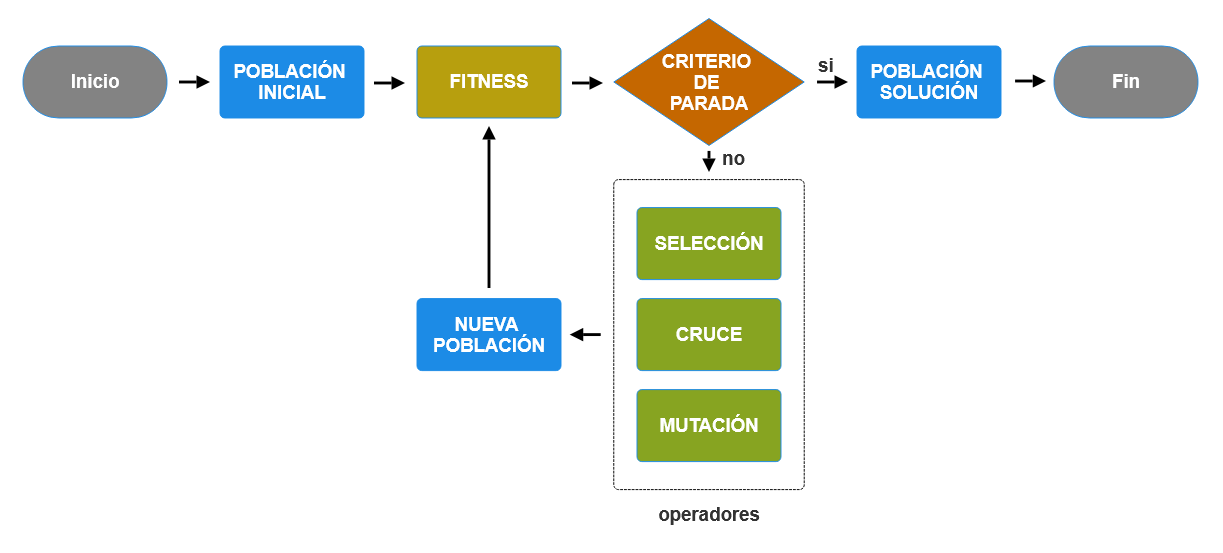
\includegraphics[width=1\textwidth]{figures/algoritmo-genetico.png}
    \caption{Algoritmo genético simple.}
    \label{fig:algoritmo-genetico}
  \end{figure}

Explicado el concepto general, se va a desglosar cada una de las fases de la figura \ref{fig:algoritmo-genetico}, que muestra el esquema básico de un algoritmo genético.

\section{Población}

Antes de explicar la generación de una población inicial, es necesario conocer algunos conceptos que son usados para representar y entender las soluciones. Son términos utilizados en la biología y en el campo de la genética. 

\begin{itemize}
    \item \textbf{Gen.} Es la unidad básica de información en un cromosoma. En una cadena de bits que representa una solución, cada bit puede considerarse un gen. En el caso que se trata en este PFG, el menú semanal, cada tipo de comida se podría considerar un gen. Por ejemplo, un gen sería bebida, plato principal o postre.
    \item \textbf{Alelo.} Es la forma específica o valor que puede tomar un gen. Siguiendo el ejemplo de bebida, posibles alelos serían agua, té o cerveza.
    \item \textbf{Cromosoma.} Es una colección de genes y representa una solución completa al problema de optimización. El cromosoma es la cadena de bits completa. En nuestro caso, la lista completa de alimentos seleccionados para una semana es el cromosoma. 
    \item \textbf{Fenotipo.} Es la manifestación real de la solución codificada. En el PFG sería cómo se preparan y sirven estos alimentos en la realidad.
\end{itemize}

En la figura \ref{fig:cromosoma} se expone la estructura de un cromosoma con el ejemplo del menú semanal de comida.

\begin{figure}[H]
  \centering
  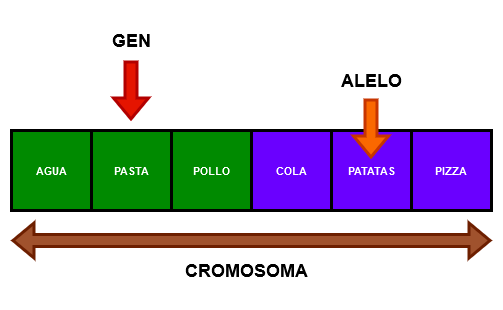
\includegraphics[width=0.625\textwidth]{figures/cromosoma.png}
  \caption{Estructura de un cromosoma.}
  \label{fig:cromosoma}
\end{figure}
\newpage
La generación de una población inicial implica crear un conjunto de soluciones candidatas. Generalmente, los individuos son seleccionados aleatoriamente dentro de los límites definidos en cada problema, asegurando que todas las áreas del espacio de búsqueda puedan ser exploradas. También existen métodos alternativos de generación que aplican ciertas restricciones para formar soluciones iniciales más prometedoras. Tomando de ejemplo el menú semanal, el espacio de búsqueda comprendería la base de datos en la que aparecen todos los alimentos con sus respectivas calorías y macronutrientes. 

\section{Evaluación}
\label{ch:evaluacion}

Se mide lo bueno que es un individuo para nuestros propósitos (la calidad del individuo). Lo más importante es definir una función de fitness correcta y representativa del problema a evaluar. Si se trata de un problema multiobjetivo, se tendrá que diseñar una función de fitness diferente por cada objetivo.

Según vayan pasando generaciones, la población inicial irá evolucionando hacia poblaciones candidatas que presentarán una mejor aptitud. Si la población ha alcanzado el objetivo, la condición de parada se activará, convirtiendo el conjunto de individuos candidatos en la población óptima. En caso de no alcanzarlo, seguirá evolucionando hacia otra población candidata distinta.

Para diseñar una función de fitness acorde al problema y al objetivo (u objetivos) se pueden seguir los siguientes pasos:

\begin{enumerate}
  \item Determinar si el objetivo es maximizar o minimizar un valor específico. En el caso que se trata en este proyecto, se busca que la diferencia entre las calorías necesarias y la suma de las calorías de los alimentos sea la menor posible, por lo que se trataría de un problema de minimización.
  \item Identificar las restricciones. En el ejemplo de los alimentos, una podría ser los límites superior e inferior de calorías permitidas.
  \item Definir la función matemática que represente el objetivo del problema. Si existen múltiples objetivos, se pueden ponderar.
  \item Incorporar las penalizaciones para soluciones que no cumplan con las restricciones.
\end{enumerate}

Por lo tanto, la mejor solución debería recibir la mejor evaluación. Esto ayudará al algoritmo a entender el camino a seguir, ya que penalizará las soluciones no factibles.

\subsection{Restricciones}
\label{ch:restricciones}

Uno de los apartados a destacar cuando se diseña la función de calidad es entender cómo se manejan las restricciones para asegurar que las soluciones generadas sean viables y de alta calidad.

Existen tres tipos de restricciones que limitan el espacio de soluciones válidas. Sea \textit{x} las variables del problema:

\begin{itemize}
  \item Restricciones de igualdad. $h_j(x) = 0$
  \item Restricciones de desigualdad. $g_k(x) \geq 0$ ó $g_k(x) \leq 0$
  \item Restricciones de contorno o de caja (\textit{box-constraints}). $x^L \leq x \leq x^U$
\end{itemize}

Estos tipos de restricciones se pueden tratar mediante distintos métodos, que también son probados de manera práctica en el apartado \ref{ch:manejo-restricciones}. En el trabajo de Carlos A. Coello (2022)~\cite{coello2022} se hace un recopilatorio de algunos de los métodos más usados y sus consiguientes ventajas y desventajas. Los más importantes son:

\begin{itemize}
  \item \textbf{Funciones de penalización.} Se penalizan las soluciones no factibles. Estas penalizaciones representan cómo de lejos está la solución de la región factible. Se transforma un problema con restricciones en uno sin restricciones utilizando una función objetivo de penalización:
  
  \[
  F(x) = f(x) + \sum_{j=1}^{m} R_j \cdot p_j(x)^\beta
  \]
  
  \begin{itemize}
    \item \( f(x) \) es la función objetivo original que se desea optimizar.
    \item \( R_j \) es un parámetro de penalización definido por el usuario para la restricción \( c_j(x) \), cuya función de penalización es \( p_j(x) \)
    \item \( \beta \) (comúnmente 1 o 2) es una constante definida por el usuario que determina cómo se pondera la violación de la restricción en la función de penalización.
    \item En problemas de maximización la suma se convierte en negativa.     
  \end{itemize}

  \newpage
  Existen varios métodos de penalización:
  
    \begin{itemize}
      \item \textbf{Penalización estática.} Se usa un valor fijo \( R_j \). Se puede ver su implementación en el problema del PFG en el punto \ref{ch:penalizacion-estatica}.
      \item \textbf{Penalización dinámica.} Se usa un factor \( R = (C \cdot t) ^ {\alpha} \), donde \( C \) y \( \alpha \) son constantes y \( t \) es el número de iteración.
      \item \textbf{Penalización adaptativa.} La penalización se adapta en función de la factibilidad de las soluciones.
    \end{itemize}
  \item \textbf{Separatista.} Dividen el problema en subproblemas más manejables que se pueden resolver por separado y luego combinar. Las restricciones y los objetivos se tratan de forma separada. Un método separatista se trata en el punto \ref{ch:metodo-separatista}.
  \begin{comment}
  \item \textbf{Preservación de la factibilidad.} Se usan representaciones especiales (codificación binaria, entera, real, etc.) que simplifican la forma del espacio de búsqueda y operadores que mantienen la factibilidad de las soluciones, lo que elimina las soluciones inválidas en cada etapa del algoritmo.
  \end{comment}
  \item \textbf{Reparación.} Se modifican las soluciones candidatas inviables de forma que no violen las restricciones.
\end{itemize}

\subsection{Condición de parada}

Tras la evaluación de calidad la condición de parada determina cuándo el algoritmo debe detenerse y presentar la solución. Si bien existe una gran variedad de condiciones de parada, las más comunes son:

\begin{itemize}
  \item Aptitud del individuo. El algoritmo se detiene si se alcanza una solución, ya sea alcanzando el valor objetivo o estando dentro de unos umbrales predefinidos.
  \item Número máximo de generaciones. El algoritmo se detiene si la población ha evolucionado un número de veces predefinido.
  \item Tiempo máximo de ejecución. Se detiene si el tiempo de ejecución es demasiado elevado.
  \item Convergencia. La ejecución puede detenerse si la población muestra poca o ninguna mejora en la aptitud durante un número determinado de generaciones consecutivas.
\end{itemize}
\newpage
\section{Operadores}

Son los procesos que se aplican a poblaciones de individuos para desarrollar generaciones futuras. Sirven para la exploración del espacio de soluciones y para la mejora de las poblaciones a través de las generaciones. Se busca que el conjunto de individuos presente una alta diversidad, ya que si es baja se corre el riesgo de caer en mínimos locales, lo que no permitiría explorar el espacio de soluciones ampliamente. En la figura \ref{fig:operadores} aparecen los operadores básicos en los algoritmos evolutivos, que son los que se van a explicar en más detalle.

\begin{figure}[H]
  \centering
  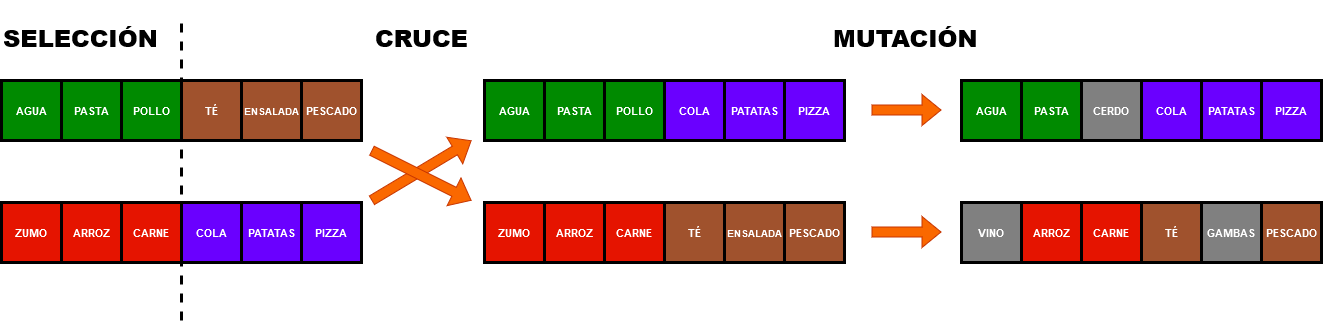
\includegraphics[width=1\textwidth]{figures/operadores.png}
  \caption{Operadores.}
  \label{fig:operadores}
\end{figure}

\subsection{Selección}
\label{Seleccion}

El primero de los operadores básicos. Elige un individuo para reproducirlo. Comúnmente, se busca un equilibrio entre la diversidad y la convergencia. El algoritmo debe explorar el espacio de búsqueda en amplitud, ya que podría caer en mínimos locales si la población es muy parecida entre sí, lo que no permitiría encontrar buenas soluciones. Pero también es de interés que las poblaciones candidatas vayan evolucionando hacia una mayor aptitud, reconduciendo el algoritmo por zonas del espacio de búsqueda más probables de encontrar una solución.

Si bien se puede seleccionar de manera equiprobable, existen métodos basados en la aptitud del individuo que buscan respetar este equilibrio. Estos son algunos:

\begin{itemize}
  \item \textbf{Método estándar (rueda de la fortuna).} Asigna a cada individuo una probabilidad proporcional a su fitness, por lo que los más aptos tienen mayor probabilidad de reproducirse. Existe un derivado de este método en el que se normalizan las probabilidades, lo que favorece aún más a los de mayor calidad.\newpage
  \item \textbf{Método del rango.} Se ordenan los individuos según su aptitud, y la probabilidad de selección se asigna según este ránking.
  \item \textbf{Selección por torneo.} Se escoge aleatoriamente un subconjunto de individuos de la población, y el mejor de este es elegido. Este es el método de selección usado en el desarrollo del algoritmo nutricional (sección \ref{ch:explicacion-algoritmo}).
\end{itemize}

\subsubsection{Selección ambiental (Reemplazo)}

Aparte de los métodos basados en la aptitud, se puede usar usa la técnica de la selección ambiental para seleccionar aquellos individuos que puedan influir significativamente en la eficacia del algoritmo genético. Existen varios métodos de selección ambiental:

\begin{itemize}
  \item \textbf{Reemplazo generacional completo.} Método tradicional en la selección y explicado en el apartado \ref{Seleccion}. Toda la población actual es reemplazada por una nueva. Promueve altas tasas de diversidad, pero conlleva una aptitud de los individuos irregular.
  \item \textbf{Reemplazo generacional parcial (\textit{Steady-State}).} Solo una parte de la población es reemplazada en cada generación. Se promueve una mejora constante en la calidad ya que las soluciones con un fitness elevado pueden mantenerse.
  \item \textbf{Reemplazo elitista.} Escoge los mejores individuos de una generación para que se mantengan en la siguiente. Esto ayuda a que la calidad del mejor individuo de una generación sea siempre igual o superior a su equivalente de la generación anterior, consiguiendo una progresión constante hacia la solución óptima, es decir, una mayor convergencia.
  \item \textbf{Selección $(\mu,\lambda)$.} De $\mu$ padres se generan $\lambda$ hijos. Los $\mu$ mejores de los $\lambda$ hijos forman la siguiente generación de padres. Es decir, si se tiene 50 padres $(\mu)$ y se generan 100 descendientes $(\lambda)$, se seleccionan los 50 mejores de los 100 descendientes para la siguiente generación.
  \item \textbf{Selección $(\mu+\lambda)$.} Igual que en la anterior, de $\mu$ padres se generan $\lambda$ hijos, pero en este caso los $\mu$ mejores de la combinación entre los $\mu$ padres y los $\lambda$ hijos forman la siguiente generación. En este caso, con el mismo ejemplo de los 50 padres y los 100 descendientes, se seleccionan los 50 de los 150 individuos combinados para la siguiente generación.
\end{itemize}

\subsection{Cruce}

Se combina el material genético de dos individuos, padres, para producir descendencia, hijos. Es decir, se utiliza para intercambiar características de dos soluciones parentales, con el objetivo de generar nuevas soluciones. Se aplica con probabilidad \(P_c\) . Al promover la mezcla de genes, ayuda a aumentar la diversidad y la convergencia, gracias a la generación de nuevos descendientes con características deseables. Se usan distintos métodos:

\begin{itemize}
  \item \textbf{Cruce de un punto.} Como se muestra en la figura \ref{fig:cruce}, se selecciona aleatoriamente una posición en el cromosoma. Todos los genes que están antes de este punto se intercambian con los que están después en la otra cadena, y viceversa, para producir dos nuevos descendientes.
  
  \begin{figure}[H]
    \centering
    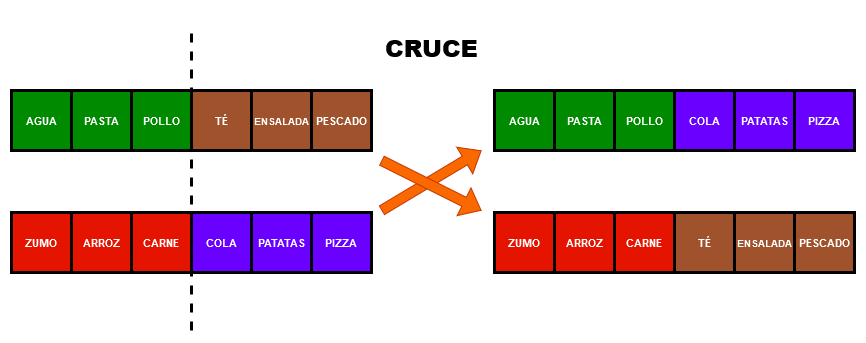
\includegraphics[width=1\textwidth]{figures/cruce.png}
    \caption{Cruce de un punto.}
    \label{fig:cruce}
  \end{figure}

  \item \textbf{Cruce de dos puntos.} Similar al cruce de un punto, pero se seleccionan dos puntos de corte. Las cadenas de genes entre estos dos puntos se intercambian entre los dos padres.
  \item \textbf{Cruce uniforme.} Cada gen tiene una probabilidad igual de ser elegido de uno de los dos padres.
\end{itemize}
\newpage
\subsection{Mutación}

Último de los operadores básicos. Se recorre toda la cadena, mutando cada gen con probabilidad \(P_m\) , es decir, eligiendo un nuevo valor mediante una elección equiprobable dentro del alfabeto. La mutación aumenta la diversidad y ayuda a no caer en mínimos locales. Algunos de los métodos usados son:

\begin{itemize}
  \item \textbf{Mutación uniforme.} Cada gen puede cambiar a otro valor con probabilidad \(P_m\), como se expone en la figura \ref{fig:mutación}.

  \begin{figure}[H]
    \centering
    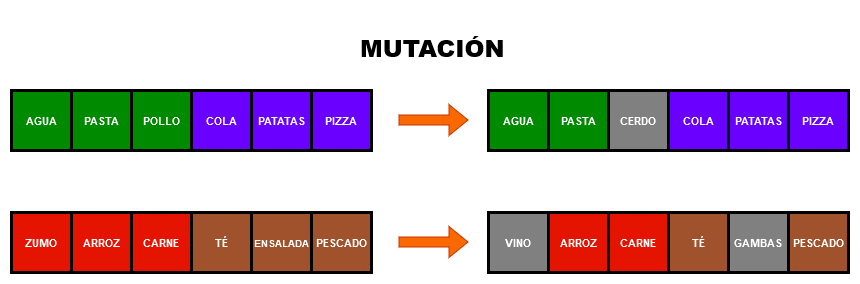
\includegraphics[width=1\textwidth]{figures/mutacion.png}
    \caption{Mutación uniforme.}
    \label{fig:mutación}
  \end{figure}

  \item \textbf{Mutación por intercambio.} Dos genes aleatorios en el cromosoma son seleccionados y sus posiciones se intercambian. 
\end{itemize}

\section{Tipos de algoritmo}

Si bien existen casos en los que solo es necesaria la optimización de un objetivo, existe una gran diversidad de problemas en la que pueden aparecer varios que se deben maximizar o minimizar. Debido a esto, existe una clasificación de los problemas según el número de objetivos a optimizar. Destacan dos grandes grupos: los problemas de optimización con un solo objetivo o \textit{Single-objective Optimization Problem (SOP)}, y los problemas de optimización multiobjetivo o \textit{Multi-objective Optimization Problem (MOP)}.

\subsection{Single-objective Optimization Problem (SOP)}

Los algoritmos que resuelven problemas \textit{SOP} se enfocan en optimizar una única función objetivo. La meta es encontrar la mejor solución posible según se busque maximizar o minimizar la función. Se usan algoritmos mono-objetivo cuando existe un único criterio de éxito.

Los algoritmos mono-objetivo presentan una función objetivo que asigna un valor numérico a cada solución, indicando su calidad. Cada solución está representada por un vector de variables de decisión, que son los parámetros que se pueden ajustar dentro del espacio de decisión. Estas soluciones deben pertenecer al conjunto factible, que incluye aquellas que cumplen con todas las restricciones del problema.

El algoritmo más usado para los problemas mono-objetivo es el \textit{''Genetic Algorithm'' (GA)}, cuyo funcionamiento sigue los pasos explicados a lo largo del capítulo \ref{ch:marco-teorico}. Destaca por su simplicidad y su capacidad para explorar grandes espacios de búsqueda.

\subsection{Multi-objective Optimization Problem (MOP)}

Los algoritmos multi-objetivo buscan optimizar múltiples funciones simultáneamente. La meta es encontrar un conjunto de soluciones que represente un equilibrio entre los distintos criterios de éxito, conocido como conjunto de Pareto.

Una solución se considera no dominada si no existe otra que mejore en, al menos, uno de los objetivos sin empeorar en los demás. El conjunto de todas las soluciones no dominadas se conoce como el conjunto de Pareto, como se ha mencionado antes.

Al igual que en los mono-objetivo, cada solución está representada por un vector de variables de decisión. Estas soluciones deben pertenecer también al conjunto factible. La diferencia se encuentra en la existencia de múltiples funciones objetivo que asignan valores numéricos a cada solución, indicando su calidad en diferentes dimensiones según el número de objetivos.

Algunos de los algoritmos más usados para los \textit{MOP} son el \textit{''Non-dominated Sorting Genetic Algorithm II'' (NSGA-II)}, el \textit{''Strength Pareto Evolutionary Algorithm 2'' (SPEA2)} o el \textit{''Multi-Objective Evolutionary Algorithm based on Decomposition'' (MOEA/D)}. Usan criterios basados en Pareto para evaluar, clasificar y seleccionar las soluciones. Buscan dispersar las soluciones para aumentar la diversidad y explorar el espacio de soluciones. Aun así, presentan grandes diferencias a la hora de desarrollar el algoritmo evolutivo.

\subsubsection{Non-dominated Sorting Genetic Algorithm II (NSGA-II)}
\label{ch:nsga2}

Este algoritmo sigue el funcionamiento general de un algoritmo genético, pero presenta ciertas modificaciones para los algoritmos multi-objetivo, como se muestra en la figura \ref{fig:nsga2}. Tras realizar la evaluación, las soluciones se ordenan en diferentes frentes de Pareto. En el primer frente se encuentran las soluciones no dominadas, en el segundo las soluciones dominadas solo por soluciones del primer frente, y así sucesivamente. Tras esto, se calcula el \textit{''crowd distance''}, una medida usada para preservar la diversidad de las soluciones. Se evalúa cómo de cerca están las soluciones entre sí en el mismo frente. Cuanto mayor sea la distancia, más aislada y diversa es la solución, lo que ayuda a explorar en profundidad el espacio de soluciones.

\textit{NSGA-II} usa elitismo, ya que combina la población de los padres y los descendientes y escoge a los mejores individuos para la siguiente generación basados en la clasificación de Pareto y en el \textit{''crowding distance''}. Además, se hace uso de la selección por torneo para elegir a los padres que se usarán en la reproducción, también usando de referencia las medidas antes citadas.

\begin{figure}[H]
  \centering
  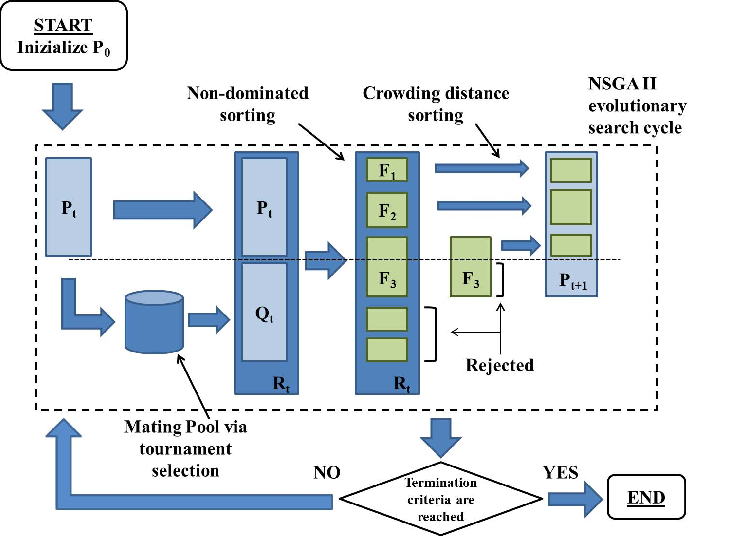
\includegraphics[width=0.8\textwidth]{figures/nsga2.png}
  \caption{Estructura general del algoritmo NSGA-II. Fuente \cite{nsga2_imagen}}
  \label{fig:nsga2}
\end{figure}

\subsubsection{Strength Pareto Evolutionary Algorithm 2 (SPEA2)}
\label{ch:spea2}

El \textit{SPEA2} también está optimizado para problemas multi-objetivo y, al igual que el NSGA-II, tiene modificaciones respecto al funcionamiento básico del algoritmo genético.

En la evaluación, a cada solución se le asigna una fuerza que refleja el número de soluciones que domina, como se expone en la figura \ref{fig:spea2}. Tras esto, se usa una medida de densidad para evaluar cuán poblada está la área alrededor de cada solución. El fitness se calcula sumando la fuerza y esta medida de densidad, lo que ayuda a la diversidad de la población. En la selección se escogen aquellas soluciones que mayor fitness presentan.

\textit{SPEA2} hace uso de un archivo externo para almacenar soluciones no dominadas. Este archivo se actualiza en cada generación y mantiene un conjunto de soluciones que representan la mejor aproximación al frente de Pareto en ese momento.

Similar al \textit{NSGA-II}, este algoritmo escoge los mejores individuos de la combinación de padres y descendientes para la siguiente generación.~\cite{pymoo_spea2}

\begin{figure}[H]
  \centering
  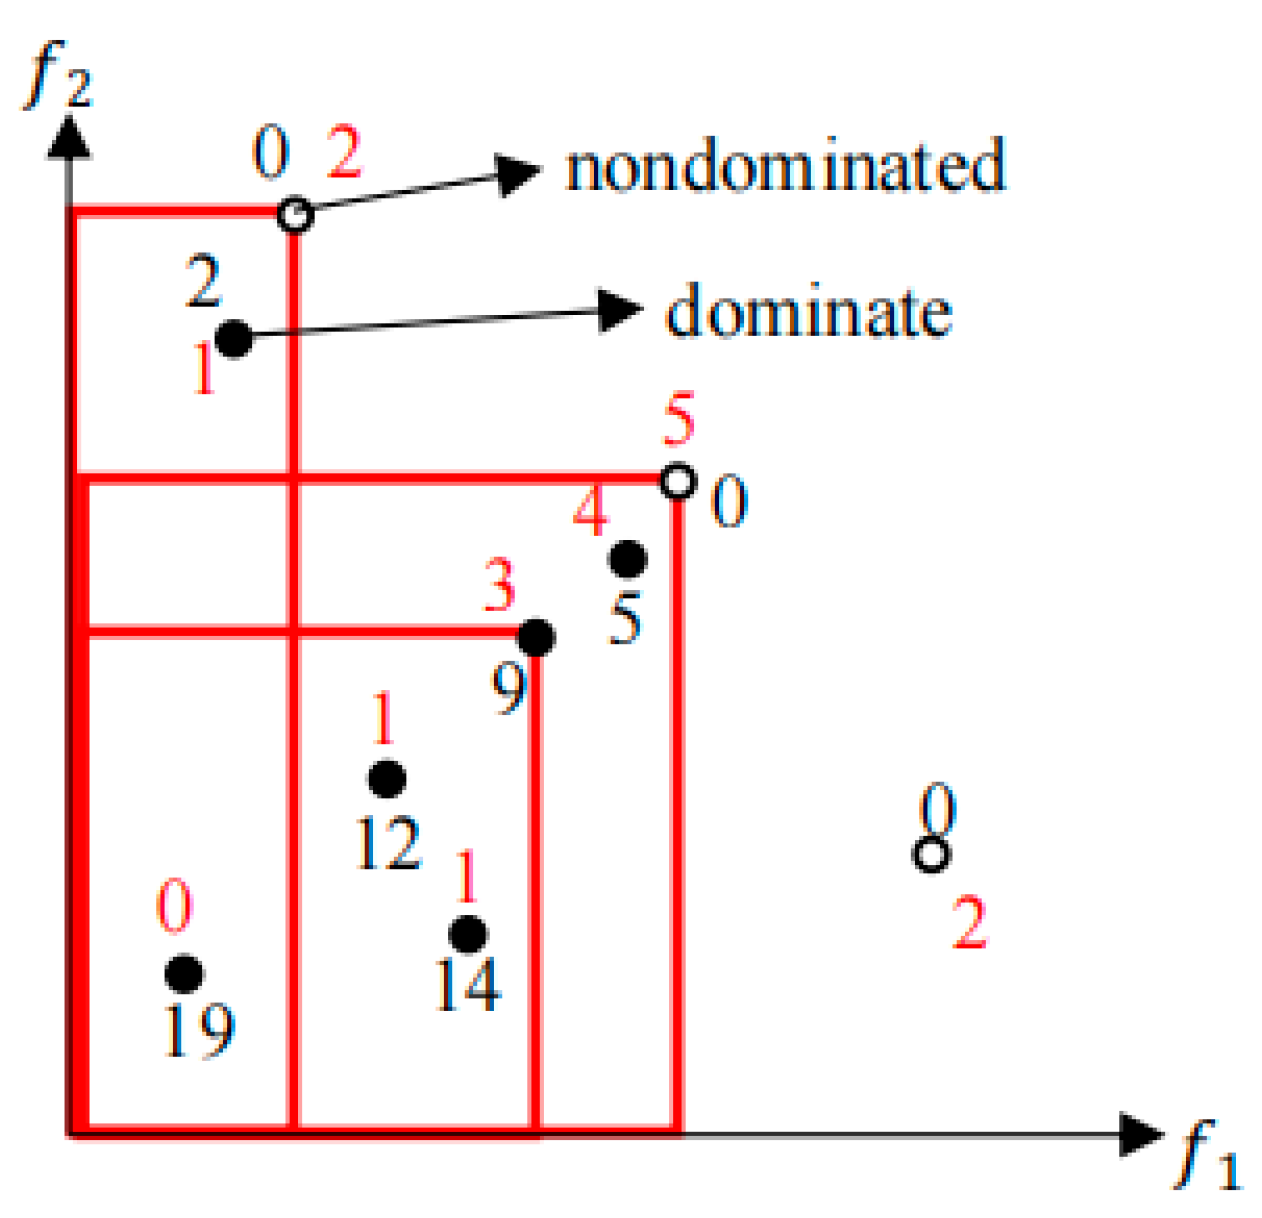
\includegraphics[width=0.5\textwidth]{figures/spea2.png}
  \caption{Cálculo del fitness en SPEA2. Fuente \cite{spea2_imagen}}
  \label{fig:spea2}
\end{figure}
\newpage
\subsubsection{Multi-Objective Evolutionary Algorithm based on Decomposition (MOEA/D)}
\label{ch:moead}

\textit{MOEA/D} hace uso de direcciones de referencia para dividir el problema multi-objetivo en problemas más pequeños de un solo objetivo. Cada dirección de referencia representa una combinación específica de los distintos objetivos. De manera ponderada, cada referencia se centra en la optimización de un objetivo particular. En el listado \ref{lst:direcciones} se muestra un ejemplo con 12 direcciones de referencia que puede ser utilizado en este proyecto, donde se busca una buena cobertura del espacio de búsqueda, que presenta 3 dimensiones (3 objetivos).

\begin{small}
\begin{lstlisting}[basicstyle=\ttfamily, caption=Direcciones de referencia.,label={lst:direcciones}]
    (1, 0, 0),          (0.67, 0.33, 0),    (0.33, 0.67, 0),
    (0, 1, 0),          (0.67, 0, 0.33),    (0.33, 0, 0.67)
    (0, 0.67, 0.33),    (0, 0.33, 0.67),    (0, 0, 1),
    (0.33, 0.33, 0.33), (0.67, 0.16, 0.16), (0.16, 0.67, 0.16)
\end{lstlisting}
\end{small}

Para generar estas direcciones existen distintos métodos, incluyendo \textit{''das-dennis''} e \textit{''incremental''}. El método \textit{''das-dennis''} es usado para distribuir uniformemente las direcciones, dividiendo el espacio en particiones equitativas. Mientras tanto, el método \textit{''incremental''} ajusta las direcciones de referencia gradualmente, permitiendo una adaptación más precisa a las áreas más prometedoras del espacio de búsqueda.

Para cada subproblema, se selecciona un número determinado de subproblemas más cercanos. Estos subproblemas forman el vecindario del primero, como se ilustra en la figura \ref{fig:moead}. Existe una probabilidad \( P_{cv} \) de que una solución se cruce con otra de su mismo vecindario. Compartir información entre vecinos ayuda a generar soluciones que cumplan cada uno de los subproblemas, por lo que son útiles para mejorar la calidad y la diversidad.~\cite{moead_pymoo}

\begin{figure}[H]
  \centering
  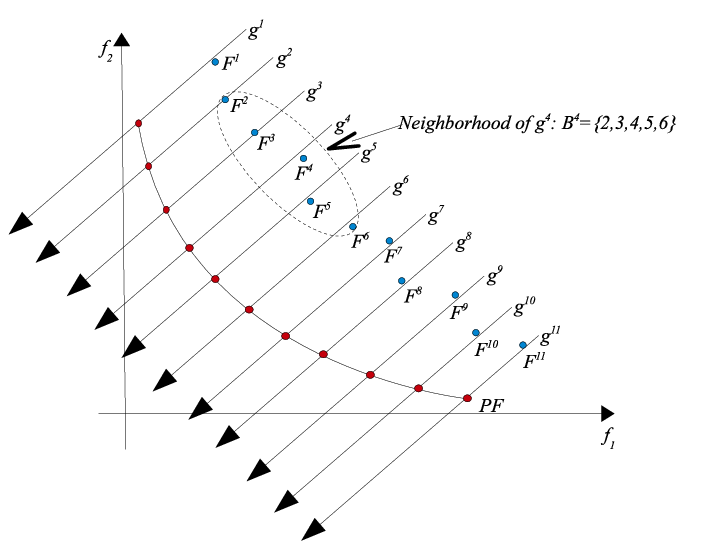
\includegraphics[width=0.73\textwidth]{figures/moead.png}
  \caption{Vecindarios en MOEA/D. Fuente \cite{moead_imagen}}
  \label{fig:moead}
\end{figure}
\begin{comment}
  \subsection{Tabla comparativa entre SOP y MOP}

  \begin{table}[h!]
    \centering
    \renewcommand{\arraystretch}{1.5}
    \begin{tabularx}{\textwidth}{|l|X|X|}
    \hline
    \textbf{Campo} & \textbf{SOP (Single-Objective Optimization)} & \textbf{MOP (Multi-Objective Optimization)} \\
    \hline
    \textbf{Función objetivo} & Una única función objetivo & Varias funciones objetivo \\
    \hline
    \textbf{Meta} & Optimizar una solución & Balancear múltiples soluciones \\
    \hline
    \textbf{Solución} & Mejor solución única & Conjunto de Pareto \\
    \hline
    \textbf{Criterio} & Un criterio de éxito & Varios criterios de éxito \\
    \hline
    \textbf{Evaluación} & Valor numérico único & Valores numéricos múltiples \\
    \hline
    \textbf{Algoritmos comunes} & GA & NSGA-II,SPEA2,MOEA/D \\
    \hline
    \textbf{Búsqueda} & Explora grandes espacios de búsqueda & Usa criterios de Pareto para explorar el espacio de soluciones \\
    \hline
    \textbf{Clasificación} & - & Basada en dominancia \\
    \hline
    \textbf{Factibilidad} & Cumplir restricciones & Cumplir restricciones \\
    \hline
    \end{tabularx}
    \caption{Comparación entre SOP y MOP.}
    \label{table:sopvsmop}
  \end{table}

\end{comment}
\chapter{Desarrollo}
\label{ch:desarrollo}

\lstdefinestyle{sqlstyle}{ % Configuración global de listings
    language=SQL,
    keywordstyle=\color{myblue},
    commentstyle=\color{darkgreen},
    stringstyle=\color{myorange},
    basicstyle=\ttfamily,
    morekeywords={CREATE, DATABASE, USE, ALTER, TABLE, ADD, COLUMN, UPDATE, SET, CHAR, INT, PRIMARY, KEY, NOT, NULL, SUBSTRING, VARCHAR, AUTO_INCREMENT},
    literate={0}{{{\color{myorange}0}}}{1}
             {1}{{{\color{myorange}1}}}{1}
             {2}{{{\color{myorange}2}}}{1}
             {3}{{{\color{myorange}3}}}{1}
             {4}{{{\color{myorange}4}}}{1}
             {5}{{{\color{myorange}5}}}{1}
             {6}{{{\color{myorange}6}}}{1}
             {7}{{{\color{myorange}7}}}{1}
             {8}{{{\color{myorange}8}}}{1}
             {9}{{{\color{myorange}9}}}{1},
}

\section{Base de datos}

\subsection{Selección de la base de datos}
La base de datos de alimentos y platos utilizada para el desarrollo del algoritmo es la perteneciente al gobierno del Reino Unido. El proyecto proporciona información detallada sobre la composición nutricional de los alimentos consumidos comúnmente en Reino Unido.~\cite{cofid2021}

La base de datos ``\textit{Composition of foods integrated dataset (CoFID)}`` se originó a partir del trabajo de Widdowson y McCance en la década de 1940 y ha sido periódicamente actualizada desde entonces para reflejar los últimos cambios en la dieta y las nuevas investigaciones científicas. La última actualización se publicó en marzo de 2021.

La elección de esta base de datos se basa en la gran cantidad de datos nutricionales que se aportan sobre los alimentos, junto con una documentación detallada para entender el trabajo. A todo esto hay que sumar la facilidad para la exportación, que permite modificarla y analizarla con suma sencillez.

CoFID incluye más de 2500 alimentos, cada uno de ellos categorizado según su grupo alimenticio. Cada alimento incorpora información sobre una amplia gama de nutrientes, como vitaminas, minerales, azúcares y otros componentes, además de los macronutrientes (carbohidratos, proteínas y grasas), que van a ser los principalmente usados en este PFG.

En la página web se pueden encontrar principalmente dos archivos. El primero es una guía de usuario en formato PDF que explica en detalle en qué consiste la base de datos y la información que se va a encontrar en ella.\newpage El segundo archivo trata de una hoja de cálculo de Microsoft Excel donde se encuentra toda la información nutricional relativa a 2.887 alimentos. Existen múltiples casos donde un mismo alimento se presenta con diferentes tipos de cocción o de aliño, lo que cambia los valores nutricionales y se considera como dos alimentos o platos distintos.

La información necesaria se encuentra en la tabla ``\textit{1.3. Proximates}``, que es donde se localizan los campos que se van a usar: \textit{''Food Code''}, identificador del alimento; \textit{''Food Name''}, nombre del alimento; \textit{''Group''}, categoría alimenticia a la que pertenece; \textit{''Protein(g)''}, que muestra los gramos de proteína por cada \textit{100g} del alimento; \textit{''Fat(g)''}, lo mismo que la proteína, pero con la grasa; \textit{''Carbohydrate(g)''}, al igual que los dos últimos campos, muestra datos de los hidratos de carbono o carbohidratos; y \textit{''Energy(kcal)''}, que representa las kilocalorías del alimento por cada \textit{100g}.

Como se puede comprobar por las descripciones previas, todos los datos están representados en base a \textit{100} gramos del alimento correspondiente. Esto también ocurre con las bebidas, cuyos valores nutricionales se han calculado en base \textit{100} mililitros. La planificación nutricional se realizará usando estas proporciones.

Por último, destacar que, debido a que la información es extraída de una web oficial del Reino Unido, todos los datos, incluyendo entre ellos el nombre de los alimentos o platos, están en inglés. En el menú de comidas resultante de la ejecución del algoritmo genético se mantendrá este idioma.

\subsection{Creación de la base de datos}
Tras haber seleccionado la fuente, se necesita un gestor de bases de datos para manipular los datos de forma eficiente. Para este trabajo se ha seleccionado MySQL Workbench, que dispone de una interfaz gráfica intuitiva para diseñar, modelar y administrar bases de datos MySQL.~\cite{mysqlworkbench}

Dentro del gestor, lo primero que se debe hacer es crear la base de datos. Se hace uso de sentencias SQL para ello. A la base de datos se le ha llamado \textit{''food\_database''}.

\newpage

Después de configurar la base de datos, se debe crear una tabla con los campos donde se almacenarán los valores. Mostrando en el listado \ref{lst:tabla} el código ejecutado, esta será la única tabla necesaria a lo largo del proyecto.

\begin{lstlisting}[style=sqlstyle, caption=Creación de la tabla y sus campos., label={lst:tabla}]
    CREATE DATABASE food_database;
    CREATE TABLE comida (
        id VARCHAR(10) NOT NULL,
        nombre VARCHAR(255) NOT NULL,
        grupo CHAR(3),
        proteinas FLOAT,
        grasas FLOAT,
        carbohidratos FLOAT,
        calorias INT,
        PRIMARY KEY(id)
    );
\end{lstlisting}

Ahora que la estructura ya está creada, falta introducir los datos. MySQL Workbench dispone de una herramienta para la importación desde archivos Comma Separated Values (valores separados por comas) o CSV, que permite con facilidad identificar los numerosos datos de la hoja de cálculo. Esto permite emparejar fácilmente los campos de la tabla recién creada con los del archivo CSV, como muestra la figura \ref{fig:importacion}, logrando una importación masiva de datos de manera correcta.

\begin{figure}[H]
    \centering
    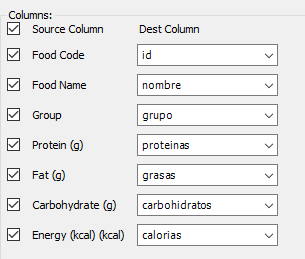
\includegraphics[width=0.4\textwidth]{figures/importacion.png}
    \caption{Importación de los datos usando MySQL Workbench.}
    \label{fig:importacion}
\end{figure}

\subsection{Cambios en la base de datos original}

Para optimizar la base de datos y mejorar el funcionamiento del algoritmo con el fin de alcanzar mejores soluciones, existen ciertos cambios a realizar a los datos aportados por el gobierno de Reino Unido.

El primer cambio es la eliminación de los datos incompletos. En la base de datos original existen diversos alimentos que no presentan toda la información que se va requerir en el trabajo. El principal promotor de este cambio es la existencia de registros que no tienen calorías asignadas (representadas en el archivo Excel con una \textit{''N''}), que han pasado con el valor \textit{0}.

Sin dejar de lado la eliminación de registros, se filtra las categorías de comidas que pueden ser ingeridas por el consumidor. Existen categorías como, por ejemplo, \textit{''Harinas, granos y almidones''} (AA) o \textit{''Grasas y aceites''} (O), que no son consumidas por el usuario como plato único, sino que participan en la cocción o en el acompañamiento del alimento principal. Por lo tanto, se eliminan. También se elimina la categoría \textit{''Bebidas Alcohólicas''} (Q), ya que sería necesario un análisis más exhaustivo y conocer las recomendaciones de los nutricionistas respecto a su consumo. De esta categoría se mantienen la cerveza, el vino, la sidra y el cava, presentes en la dieta mediterránea y de las que la Sociedad Española de Nutrición Comunitaria (SENC) recomienda el consumo opcional, moderado y responsable~\cite{senpiramide}.

También se ha modificado el grupo \textit{''Zumos''} (PE), donde \textit{PE} se ha cambiado por \textit{FE}. Se ha movido al grupo \textit{''Frutas''} (F) porque los zumos son mucho más parecidos a los alimentos de este grupo que al de las bebidas (P).

En el apéndice \ref{ch:grupos-comida} se encuentran todos los grupos con los que se va a trabajar.

Tras los cambios realizados queda un total de 2616 registros. En la figura \ref{fig:ejemplo} se puede ver un ejemplo de algunos de los alimentos.

\begin{figure}[H]
    \centering
    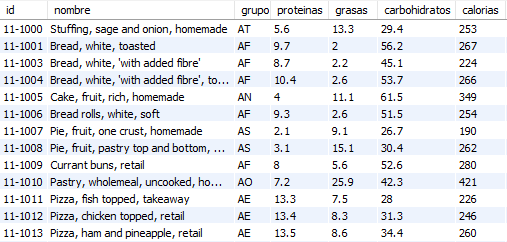
\includegraphics[width=0.65\textwidth]{figures/ejemplo.png}
    \caption{Resultado final de la base de datos.}
    \label{fig:ejemplo}
\end{figure}

\section{Conceptos nutricionales}

Se ha hecho uso de distintas fuentes para los valores nutricionales utilizados para el cálculo de los objetivos, restricciones y límites que se representan en el problema.

En el algoritmo se busca crear un menú equilibrado y personalizado para el usuario, con el propósito de mantener el peso y la masa corporal del individuo.

\subsection{Cálculo de calorías}
\label{ch:calculo-calorías}

El primer objetivo es el calórico, explicado en el apartado \ref{ch:objetivo-restriccion-calorías}. Para ello es necesario saber cuántas kilocalorías diarias necesita el usuario. La Tasa Metabólica Basal (TMB) es la cantidad de energía que el cuerpo necesita para mantener las funciones vitales en reposo. Existen diversas fórmulas de calcularla, pero en este proyecto se hace uso de una las más extendidas actualmente, la fórmula de Harris-Benedict revisada por Mifflin et al.~\cite{mifflin1990}. Esta fórmula toma en cuenta el peso, la altura, la edad y el sexo para estimar las kilocalorías.

\begin{itemize}
    \item Para hombres:
    \[
    \text{TMB} = (10 \times \text{peso en kg}) + (6.25 \times \text{altura en cm}) - (5 \times \text{edad en años}) + 5
    \]
    \item Para mujeres:
    \[
    \text{TMB} = (10 \times \text{peso en kg}) + (6.25 \times \text{altura en cm}) - (5 \times \text{edad en años}) - 161
    \]
\end{itemize}

Como se explica en la definición de la TMB, esta energía es calculada en reposo. Por lo tanto, para alcanzar una aproximación real será necesario multiplicar el resultado por un factor que depende del nivel de actividad física.~\cite{krause2016}

\begin{itemize}
    \item Sedentario (poco o ningún ejercicio): \textit{TMB $\times$ 1.2}
    \item Actividad ligera (ejercicio ligero o deportes 1-3 días a la semana): \textit{TMB $\times$ 1.375}
    \item Actividad moderada (ejercicio moderado o deportes 3-5 días a la semana): \textit{TMB $\times$ 1.55}
    \item Actividad alta (ejercicio intenso o deportes 6-7 días a la semana): \textit{TMB $\times$ 1.725}
    \item Actividad muy alta (ejercicio muy intenso, trabajos físicos o entrenamiento dos veces al día): \textit{TMB $\times$ 1.9}
\end{itemize}

Por ejemplo, para un hombre de \textit{23 años} que pesa \textit{75 kg} y mide \textit{175 cm} su TMB sería de \textit{1734 kilocalorías por día}. Pero como también realiza una actividad moderada, habría que multiplicar por \textit{1.55}, dando un total de \textit{2687.31 kcal/día}.

\begin{comment}
\subsection{Distribución de calorías}

El segundo objetivo es la correcta distribución diaria de calorías. Se busca que los alimentos ingeridos en cada comida (desayuno, tentempié, almuerzo, merienda y cena) estén dentro de unos límites que sean recomendables. Estos límites son, siguiendo las pautas del Ministerio de Sanidad~\cite{alimentacion_saludable}:

\begin{itemize}
    \item $20\% = \% \text{ de kcal en el desayuno}$
    \item $5\% \leq \% \text{ de kcal en el tentempié} \leq 10\%$
    \item $30\% = \% \text{ de kcal en el almuerzo}$
    \item $5\% \leq \% \text{ de kcal en la merienda} \leq 10\%$
    \item $25\% \leq \% \text{ de kcal en la cena} \leq 30\%$
\end{itemize}

Para calcular el porcentaje de nuestras calorías bastaría con sumar los alimentos correspondientes a una comida en particular, dividirlo entre el número de calorías totales consumidas en ese día y multiplicar el resultado por \textit{100}. La fórmula en una comida como el almuerzo es:
\[
\left( \frac{\text{kcal alimento 1} + \text{kcal alimento 2} + \text{kcal bebida}}{\text{kcal totales}} \right) \times 100
\]
\end{comment}

\subsection{Distribución de macronutrientes}
\label{ch:distribucion-macronutrientes}

Otro objetivo, tratado en el punto \ref{ch:objetivo-restriccion-macronutrientes}, es la correcta distribución diaria de macronutrientes: hidratos de carbono, proteínas y grasas. El \textit{Institute of Medicine (IOM)}, en su trabajo de 2005~\cite{iom2005}, define los AMDR (Acceptable Macronutrient Distribution Ranges) como los rangos de ingesta para macronutrientes que se asocian con un riesgo reducido de enfermedades crónicas y aseguran una ingesta adecuada de nutrientes esenciales. Estos límites para adultos son:

\begin{itemize}
    \item $45\% \leq \% \text{ de carbohidratos} \leq 65\%$
    \item $10\% \leq \% \text{ de proteínas} \leq 35\%$
    \item $20\% \leq \% \text{ de grasas} \leq 35\%$
\end{itemize}

Para verificar si la solución respeta estos límites, primero es necesario calcular cuántas kilocalorías aporta cada macronutriente. Siguiendo el estudio del \textit{IOM}, las kilocalorías por gramo de cada macronutriente son:

\begin{itemize}
    \item Carbohidratos: \textit{4 kcal} por gramo
    \item Proteínas: \textit{4 kcal} por gramo
    \item Grasas: \textit{9 kcal} por gramo
\end{itemize}

La suma de las kilocalorías individuales de cada macronutriente equivale al total de calorías del alimento, dato del que ya se dispone.

Con las kilocalorías de cada macronutriente ya calculadas, solo falta dividir estas entre las calorías totales y multiplicarlo por \textit{100} para saber los porcentajes de cada macronutriente. Por ejemplo, para calcular el porcentaje de carbohidratos sería:
\[
\left( \frac{\text{kcal de carbohidratos}}{\text{kcal totales}} \right) \times 100
\]

Siguiendo el caso de los hidratos de carbono, \textit{11 g} de carbohidratos de un alimento de \textit{98 kcal} representa un porcentaje del \textit{44.9 \%} respecto al total de calorías.


\section{Cromosoma planteado}
\label{ch:solucion-planteada}

Se ha buscado plantear un menú siguiendo los hábitos alimenticios y nutricionales de los consumidores españoles.

La primera parte es la elección de la estructura del cromosoma solución. En este problema se ha planteado que cada gen represente un alimento diferente consumido. Como se muestra en la figura \ref{fig:cromosoma_desarrollo}, cada día del menú semanal incluye 5 comidas: desayuno, tentempié, almuerzo, merienda y cena. De estas comidas, las tres principales, el desayuno, el almuerzo y la cena, consta cada una de 2 alimentos y 1 bebida, haciendo un total de 3 genes. Las otras dos comidas, tentempié y merienda, consideradas como comidas entre horas, contienen 1 alimento cada una, sumando 2 genes adicionales al cromosoma.

Cada día presenta al final 11 genes (o alimentos). Como el proyecto trata de una planificación semanal, se repite esta cadena por cada día de la semana, dando un cromosoma que presenta un total de 77 genes.

\begin{figure}[H]
    \centering
    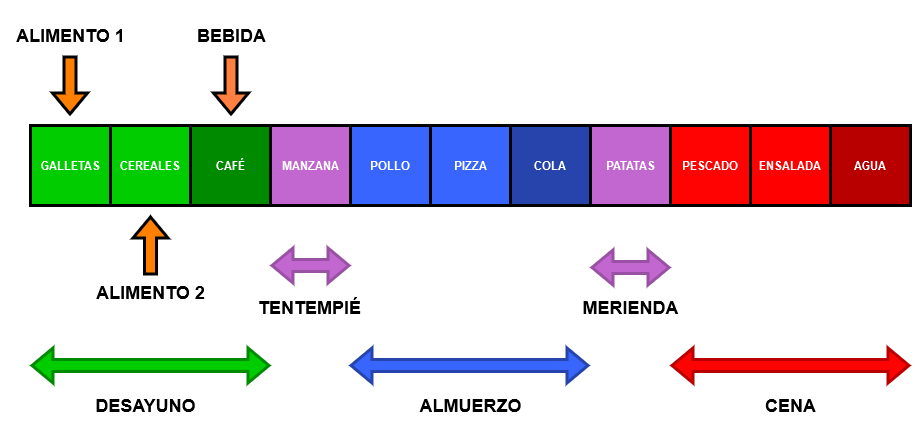
\includegraphics[width=1\textwidth]{figures/cromosoma_desarrollo.png}
    \caption{Estructura de la solución.}
    \label{fig:cromosoma_desarrollo}
\end{figure}

Como se ha explicado, el tercer gen de cada comida principal está reservado para una bebida, por lo que es necesario filtrar los grupos de comida para que seleccione solo un alimento de esta categoría. Estos cambios que se realizan en la inicialización y mutación son explicados en el apartado \ref{ch:explicacion-algoritmo}, pero primero se define qué categorías de alimentos (detalladas en el apéndice \ref{ch:grupos-comida}) están reservadas para ciertos genes o comidas.

\begin{itemize}
    \item El tercer gen de cada comida principal está destinado a una bebida. De las categorías disponibles, solo se pueden seleccionar de los grupo \textit{''Bebidas''} (P), \textit{''Jugos de frutas''} (FC), \textit{''Zumos''} (FE) o \textit{''Bebidas Alcohólicas''} (Q) (solo si el sujeto es mayor de edad).
    \item Debido a que la bebida del desayuno suele ser una bebida con leche (no presente en el grupo \textit{P}), café o un zumo, se ha decidido que este gen sea de las categorías \textit{''Leche de vaca''} (BA), \textit{''Bebidas a base de leche''} (BH), \textit{''Bebidas en polvo, esencias e infusiones''} (PA), \textit{''Jugos de frutas''} (FC) o \textit{''Zumos''} (FE).
    \item También los alimentos del desayuno suelen diferenciarse con respecto a los del almuerzo y la cena, que son comúnmente intercambiables entre sí. Por ello, los alimentos de esta comida son del grupo \textit{''Huevos''} (C), \textit{''Frutas''} (FA), \textit{''Bacon''} (MAA) o \textit{''Cereales''} (A), excepto \textit{''Arroz''} (AC), \textit{''Pasta''} (AD) y \textit{''Pizza''} (AE), que se suelen consumir en el almuerzo o la cena.
    \item Para las comidas entre horas (tentempié y merienda), se seleccionan alimentos de las categorías \textit{''Frutas''} (F) y \textit{''Azúcares''} (S).
    \item Para las otras dos comidas principales, el almuerzo y la cena, los alimentos pueden ser de cualquier grupo, excepto los cereales, salvo \textit{''Panes''} (AF) y las excepciones antes mencionadas: el arroz, la pasta y las pizzas.
\end{itemize}


\section{Objetivos y restricciones}
\label{ch:objetivo-restricciones}
\begin{comment}
Para los objetivos se crean funciones de minimización, donde la solución candidata (o soluciones) con el valor más bajo es la que mayor aptitud presenta.
\end{comment}
\subsection{Objetivo y restricción de calorías}
\label{ch:objetivo-restriccion-calorías}

El primer objetivo introducido en el problema es de las kilocalorías. Se busca que la diferencia entre las kilocalorías que el usuario necesita diariamente y la suma de las kilocalorías de todos los alimentos consumidos en un día sea 0 ó lo más cercano posible. La función de evaluación mide cuánto se ha desviado en total en toda la semana, es decir, se va sumando cada desviación de kilocalorías diaria hasta obtener un valor semanal.

Se consulta al usuario por distintos atributos físicos y su nivel de actividad, con los cuales se calcula la tasa metabólica basal y, en última instancia, las kilocalorías, como se explica en el apartado \ref{ch:calculo-calorías}.
\newpage
El objetivo está atado a una restricción \textit{box-constraint}. Se penalizan aquellas desviaciones diarias que superen los límites superior e inferior del 10\% respecto a las kilocalorías que el usuario necesita. Busca que las soluciones que se alejen bastante del objetivo sean menos seleccionadas.
\begin{small}
\[
    \begin{aligned}
    & \text{Minimizar } f_{\text{calorías}}(c_{i,d}) = \sum_{d=1}^{7} \left| k - \sum_{i=1}^{n_d} c_{i,d} \right| \\
    & \text{Sujeto a } 0.9k \leq \sum_{i=1}^{n_d} c_{i,d} \leq 1.1k, \quad \forall d \in \{1, 2, \ldots, 7\}
    \end{aligned}
    \]

        Donde:
        \begin{itemize}
        \item \( c_{i,d} \) es la cantidad de calorías del alimento \( i \) consumido en el día \( d \).
        \item \( k \) es el objetivo calórico diario.
        \item \( n_d \) es el número total de alimentos consumidos en el día \( d \).
        \end{itemize}
\end{small}


\subsection{Objetivo y restricción de macronutrientes}
\label{ch:objetivo-restriccion-macronutrientes}

Este objetivo trata de distribuir correctamente los macronutrientes a lo largo del día. Se busca que cada tipo de macronutriente se encuentre dentro de los límites recomendados en el apartado \ref{ch:distribucion-macronutrientes}, poniendo como objetivo la media de estos límites. Similar al anterior objetivo, se calcula la diferencia diaria entre estas medias y los valores reales de proteínas, carbohidratos y grasas obtenidos. Posteriormente, la función evalúa la desviación semanal total.

Existe también una restricción de caja asociada a este objetivo, que exige que la ingesta diaria de cada macronutriente se mantenga dentro de los límites especificados.
\begin{small}
    \[
    \begin{aligned}
    & \text{Minimizar } f_{\text{macronutrientes}} = \sum_{d=1}^{7} \Bigg( \left| \frac{\sum_{i=1}^{n_d} C_{i,d}}{\sum_{i=1}^{n_d} E_{i,d}} - 0.55 \right| \\
    & \qquad + \left| \frac{\sum_{i=1}^{n_d} P_{i,d}}{\sum_{i=1}^{n_d} E_{i,d}} - 0.225 \right| + \left| \frac{\sum_{i=1}^{n_d} G_{i,d}}{\sum_{i=1}^{n_d} E_{i,d}} - 0.275 \right| \Bigg) \\
    & \text{Sujeto a } \\
    & \quad 0.45 \leq \frac{\sum_{i=1}^{n_d} C_{i,d}}{\sum_{i=1}^{n_d} E_{i,d}} \leq 0.65, \\
    & \quad 0.10 \leq \frac{\sum_{i=1}^{n_d} P_{i,d}}{\sum_{i=1}^{n_d} E_{i,d}} \leq 0.35, \\
    & \quad 0.20 \leq \frac{\sum_{i=1}^{n_d} G_{i,d}}{\sum_{i=1}^{n_d} E_{i,d}} \leq 0.35, \\
    & \quad \forall d \in \{1, 2, \ldots, 7\}
    \end{aligned}
    \]
\newpage
        Donde:
        \begin{itemize}
        \item \( E_{i,d} \) es la cantidad de energía (calorías) del alimento \( i \) consumido en el día \( d \).
        \item \( C_{i,d} \) es la cantidad de calorías provenientes de carbohidratos del alimento \( i \) consumido en el día \( d \).
        \item \( P_{i,d} \) es la cantidad de calorías provenientes de proteínas del alimento \( i \) consumido en el día \( d \).
        \item \( G_{i,d} \) es la cantidad de calorías provenientes de grasas del alimento \( i \) consumido en el día \( d \).
        \item \( n_d \) es el número total de alimentos consumidos en el día \( d \).
        \end{itemize}
\end{small}

\subsection{Objetivo de preferencia}

Este objetivo busca la personalización del menú incluyendo los grupos de alimentos favoritos del usuario, o excluyendo aquellos que no le gustan. Se favorecerán los grupos preferidos y se penalizarán los que no. Se puede considerar una restricción de igualdad débil, ya que penaliza las soluciones que la violan pero no las invalida. A diferencia de los otros objetivos, esta función de minimización puede alcanzar valores negativos si existe una gran variedad de alimentos con grupo predilecto en la planificación.
\[
\text{Minimizar } f_{\text{preferencia}} = \sum_{i=1}^{N}
\begin{cases} 
-P & \text{si } g(a_i) = G_+ \\
P & \text{si } g(a_i) = G_- \\
0 & \text{en otro caso}
\end{cases}
\]
\begin{small}
    Donde:
    \begin{itemize}
    \item \( f_{\text{preferencia}} \) es la penalización total de preferencia de grupo durante la semana.
    \item \( N \) es el número total de alimentos consumidos en la semana.
    \item \( a_i \) es el alimento \( i \) consumido durante la semana.
    \item \( G_+ \) es el grupo que gusta.
    \item \( G_- \) es el grupo que no gusta.
    \item \( P \) es la penalización de preferencia.
    \item \( g(a_i) \) es el grupo del alimento \( a_i \).
    \end{itemize}
\end{small}

\subsection{Restricción de alergia}

Similar al objetivo de preferencia, es una restricción de igualdad donde se penaliza severamente si el usuario es alérgico al grupo del alimento del menú. Al finalizar la semana, se suman todas las penalizaciones de alergias, haciendo que sea inviable para el algoritmo volver a seleccionar un alimento que produzca alergia.
\[
\text{Minimizar } f_{\text{alergia}} = \sum_{i=1}^{N} 
\begin{cases} 
P_{\text{alergia}}^2 & \text{si } g(a_i) = G_{\text{alergia}} \\
0 & \text{en otro caso}
\end{cases}
\]
\begin{small}
    Donde:
    \begin{itemize}
    \item \( f_{\text{alergia}} \) es la penalización total por alergia durante la semana.
    \item \( N \) es el número total de alimentos consumidos en la semana.
    \item \( a_i \) es el alimento \( i \) consumido durante la semana.
    \item \( G_{\text{alergia}} \) es el grupo al que el usuario es alérgico.
    \item \( P_{\text{alergia}} \) es la penalización fuerte por alergia.
    \item \( g(a_i) \) es el grupo del alimento \( a_i \).
    \end{itemize}
\end{small}

\section{Construcción del algoritmo}
\label{ch:explicacion-algoritmo}

El código completo se encuentra en el repositorio de Github del autor~\cite{quesada_nutritionplanning}.

La biblioteca usada para la creación del algoritmo evolutivo ha sido \textit{Pymoo}. \textit{Pymoo} es un framework de \textit{Python} diseñado para la optimización multiobjetivo. Entre sus ventajas se encuentran la amplia gama de algoritmos para abordar los problemas, como \textit{NSGA-II}, \textit{SPEA2} o \textit{MOEA/D}. Permite modificar fácilmente los operadores de selección, cruce y mutación, lo que ayuda a la personalización del algoritmo según el problema. Además, \textit{Pymoo} presenta un conjunto de herramientas de visualización para la interpretación de resultados, permitiendo entender el comportamiento de los algoritmos.~\cite{pymoo}

Se ha creado una clase personalizada que hereda de \textit{''ElementwiseProblem''}, ya que esta última proporciona una estructura eficiente para evaluar cada solución individualmente, como se muestra en el listado \ref{lst:planning}.
\newpage
\begin{lstlisting}[basicstyle=\ttfamily, caption=Clase para la evaluación.,label={lst:planning}]
    CLASE PlanningComida hereda ElementwiseProblem
    
        MÉTODO __init__(self, num_variables, limites_variables,
                            num_objetivos, num_restricciones)
            INICIALIZAR num_variables
            INICIALIZAR limites_variables
            INICIALIZAR num_objetivos
            INICIALIZAR num_restricciones
            LLAMAR al constructor de ElementwiseProblem
    
        MÉTODO evaluate(self, solución, out)
            CALCULAR valores_objetivo
            CALCULAR valores_restricciones
            out["F"] = valores_objetivo
            out["G"] = valores_restricciones
\end{lstlisting}

El primer método creado es \textit{''\_\_init\_\_''}, que inicializa los parámetros del problema, incluyendo el tamaño de la solución (77 genes), el número de objetivos y restricciones (3 cada uno) y los límites del problema (el tamaño de la base de datos).

El segundo método es \textit{''evaluate''}, que es donde se define cómo se evalúan las soluciones. Este método recibe una solución individual y calcula su aptitud a partir de los objetivos y restricciones definidos en el apartado \ref{ch:objetivo-restricciones}.

Se recorre la cadena y, por cada gen, se extraen las calorías, el grupo y los macronutrientes. Se comprueba el objetivo de la preferencia comparando el grupo del alimento con los grupos de preferencia del usuario y, en caso de ser necesario, se suma una penalización a una variable que contará todas las sanciones totales de la solución respecto a este objetivo. El mismo procedimiento se hace con la restricción de la alergia.

Por cada 11 genes de la cadena (que representa un día) se comprueba el objetivo calórico, donde la desviación de kilocalorías diarias respecto al objetivo marcado para el usuario se suma a un contador que refleja la desviación semanal total. Este es el valor a minimizar. Pero, además, existe otro contador que suma todas las penalizaciones de la restricción calórica. Cada vez que las kilocalorías diarias se sale de los límites del 10\% se agrega una penalización a este contador. Este es otro valor que se busca minimizar.

El cálculo de los valores a minimizar del objetivo y restricción de macronutrientes sigue el mismo proceso que el de las calorías.

Los resultados de las evaluaciones se almacenan en los diccionarios \textit{''out[F]''} y \textit{''out[G]''}. \textit{''out[F]''} contiene los valores de las funciones objetivos, que intentamos optimizar. \textit{''out[G]''}, muy usado en métodos separatistas para el manejo de restricciones, contiene los valores de las restricciones que deben ser satisfechas para que las soluciones se consideren factibles. Si se usase, por ejemplo, métodos de penalización para las restricciones, no sería necesario incluir \textit{''out[G]''}, ya que las restricciones se tratan como funciones objetivo. 

Tras la creación de la clase, hay que crear una función que recoja los resultados de esta clase para incluirlos en el algoritmo evolutivo. El funcionamiento del algoritmo es, en esencia, el mismo que se ha explicado en la sección \ref{ch:marco-teorico}, aunque se puede modificar o añadir algún operador según el tipo de algoritmo usado, razón de la experimentación con distintos algoritmos del apartado \ref{ch:algoritmos-multiobjetivo}. Por lo tanto, lo primero a seleccionar es el algoritmo con el que se va a trabajar, ya sea NSGA-II, MOEA/D, etc.

Se selecciona el número de individuos por generación y el número de generaciones que el algoritmo evaluará. Como no se ha puesto ninguna condición de parada específica el algoritmo terminará tras haber evaluado todas las generaciones predefinidas.

Lo primero que el algoritmo hace es crear la matriz en la que se aloja toda la población, que tiene un tamaño del número de genes (o variables) por solución multiplicado por el número de individuos de una generación. Por ejemplo, si el menú se compone de \textit{77} genes y se selecciona un tamaño de población de \textit{100} indiviudos, se crea una matriz de \(100 \, individuos \times 77 \, genes\), en la que cada solución candidata se evalúa individualmente.

\textit{Pymoo} dispone de varios métodos de incialización, entre los que destaca \textit{''IntegerRandomSampling''}, usado para la generación de matrices de enteros. Este se puede usar en el planificador de comidas al seleccionar el índice del alimento que se añade al menú, el cual es un número entero. Pero se ha decidido crear una versión modificada del mismo para que genere soluciones que sean interesantes en el contexto del proyecto. En vez de seleccionar un índice aleatorio de un alimento de la base de datos, selecciona basándose en las características propias de la solución, explicadas en el apartado \ref{ch:solucion-planteada}. Es decir, se ha configurado para que se seleccione una bebida cuando el gen sea el tercero de una comida principal o para que los alimentos del desayuno sean de la categoría \textit{''Cereales''} (A), por ejemplo. Así se consigue que la primera población de la generación cumpla las particularidades del problema, como se observa en la figura \ref{fig:matriz-inicializacion}.

\begin{figure}[H]
    \centering
    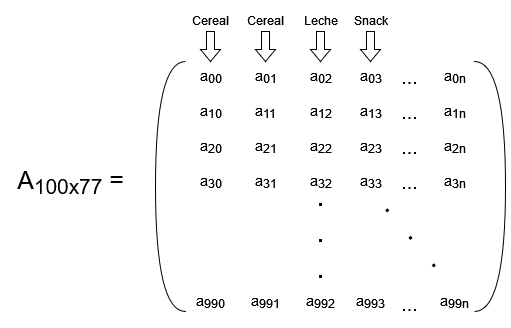
\includegraphics[width=0.75\textwidth]{figures/matriz-inicializacion.png}
    \caption{Matriz de inicialización.}
    \label{fig:matriz-inicializacion}
\end{figure}

Cada solución de esta población es evaluada según lo explicado al comienzo de este apartado. Si no ha llegado al número total de generaciones, el algoritmo se prepara para generar una nueva población a partir de los operadores.

En la selección se eligen individuos de la población basado en la aptitud. En este caso concreto los valores más bajos presentarán una mayor aptitud, al ser funciones de minimización. Se va a usar la selección por torneo, predeterminada por \textit{Pymoo} para este tipo de problemas.

Tras elegir los individuos, se cruzan para la generación de una nueva población.  Se puede variar entre el cruce de un punto y el de dos puntos, asignándoles a cada uno de ellos una probabilidad de cruce \(P_c\)  . Aparte de los mecanismos elitistas que usen los algoritmos multi-objetivo, no se ha realizado ningún método extra de selección ambiental, por lo que se realiza un reemplazo generacional completo.

Para la mutación ocurre como con la inicialización. En vez de elegir un método de los que ofrece \textit{Pymoo}, se ha decidido crear un método personalizado. El nuevo método recorre cada individuo creado en el cruce y decide si el gen es reservado para una bebida, para un snack, etc. Con una probabilidad \(P_m\) a determinar, muta una bebida por otra bebida o un alimento de una categoría determinada por otro de la misma categoría, como se muestra en la figura \ref{fig:mutacion-custom}. Esto logra, junto con la inicialización, que todas las soluciones a lo largo de las generaciones cumplan con las peculiaridades de este problema.

\begin{figure}[H]
    \centering
    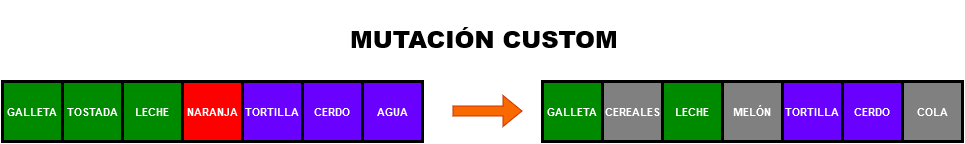
\includegraphics[width=1\textwidth]{figures/mutacion-custom.png}
    \caption{Mutación personalizada.}
    \label{fig:mutacion-custom}
\end{figure}

Por último, esta nueva población resultante vuelve a ser evaluada en busca de ser óptima para el problema.

El algoritmo evolutivo se ejecuta utilizando la función \textit{''minimize''} de \textit{Pymoo}, que toma el problema y la configuración del algoritmo. Como se muestra en la tabla \ref{tab:optimizacion}, el algoritmo va avanzando en busca de mejores soluciones.

En la tabla se aprecia, en orden: \textit{''n\_gen''} muestra el número de generación, \textit{''n\_eval''} es el contador de evaluaciones de individuos, \textit{''n\_nds''} es el número de soluciones no dominadas encontradas, \textit{''cv\_min''} es el valor mínimo de violación de una población, \textit{''n\_avg''} es el valor promedio de violación de una población, \textit{''eps''} es una métrica que mide la convergencia del algoritmo hacia soluciones óptimas e \textit{''indicator''} se usa para clasificar la calidad del frente de Pareto en cada generación.

\begin{table}[h!]
    \centering
    \small % Reduce el tamaño del texto
    \begin{tabularx}{\textwidth}{@{}ccccccc@{}}
        \toprule
        \textbf{n\_gen} & \textbf{n\_eval} & \textbf{n\_nds} & \textbf{cv\_min} & \textbf{cv\_avg} & \textbf{eps} & \textbf{indicator} \\ 
        \midrule
         1 &   100 &  1 & 2.415619E+03 & 5.717019E+03 &          - &          - \\ 
         2 &   200 &  1 & 1.789955E+03 & 4.574975E+03 &          - &          - \\ 
         3 &   300 &  1 & 1.290943E+03 & 3.787494E+03 &          - &          - \\ 
         4 &   400 &  1 & 1.195388E+03 & 3.107680E+03 &          - &          - \\ 
         5 &   500 &  1 & 1.070258E+03 & 2.478680E+03 &          - &          - \\ 
         6 &   600 &  1 & 0.000000E+00 & 1.867363E+03 & 1.0000000000 &     ideal \\ 
         7 &   700 &  2 & 0.000000E+00 & 1.400831E+03 & 0.5000000000 &     ideal \\ 
         8 &   800 &  3 & 0.000000E+00 & 9.870077E+02 & 0.2500000000 &         f \\ 
         9 &   900 &  4 & 0.000000E+00 & 6.756844E+02 & 0.1250000000 &     ideal \\ 
        10 &  1000 &  5 & 0.000000E+00 & 4.510310E+02 & 0.0625000000 &     ideal \\ 
        \bottomrule
    \end{tabularx}
    \caption{Resultados del algoritmo genético.}
    \label{tab:optimizacion}
\end{table}

El algoritmo, con este manejo de restricciones, está configurado para que, hasta que no alcance una solución viable (\textit{''cv\_min''}=0), no empieza a evaluar la convergencia y la calidad del frente de Pareto.

En el caso de que, como se ha explicado antes, no fuera necesario \textit{''out[G]''} por el manejo de las restricciones, simplemente desaparecen \textit{''cv\_min''} y \textit{''cv\_avg''}, y \textit{''n\_nds''}, \textit{''eps''} e \textit{''indicator''} se calculan desde la primera generación.

Todas las métricas que obtiene el algoritmo son guardadas en una variable \textit{''resultado''}, a la que se puede acceder.

\begin{itemize}
    \item En \textit{''resultado.X''} se encuentra una matriz que contiene las soluciones no dominadas encontradas. En este proyecto son cada uno de los posibles menús factibles que el algoritmo ha encontrado. Siguiendo el ejemplo \ref{tab:optimizacion}, en 10 generaciones el algoritmo ha encontrado 5 soluciones no dominadas, por lo que la matriz tiene un tamaño de \(5 \, n\_nds\ \times 77 \, genes\).
    \item En \textit{''resultado.F''} se encuentra una matriz que contiene los valores de las funciones objetivo para cada solución no dominada encontrada. Como el algoritmo presenta 3 objetivos, la matriz puede tener un tamaño de \(5 \, n\_nds \times 3 \, objetivos\).
    \item En \textit{''resultado.G''} se encuentra una matriz muy parecida a \textit{''resultado.F''}, pero con las restricciones en vez de los objetivos. Esta matriz se encuentra vacía si los objetivos y las restricciones no se tratan de manera separada.
\end{itemize}

\subsection{Manejo de restricciones}
\label{ch:manejo-restricciones}

\subsubsection{Penalización estática}
\label{ch:penalizacion-estatica}

En este método se penalizan las soluciones que violan las restricciones. En las funciones en las que se definen las restricciones de calorías y macronutrientes, se calcula una penalización proporcional a la diferencia entre el objetivo y los nutrientes consumidos, multiplicada por una constante de penalización, como se muestra en el listado \ref{lst:factores}. Poniendo de ejemplo la restricción de calorías, si el objetivo calórico es 2500 kilocalorías y la diferencia con las kilocalorías ingeridas está fuera del 10\%, se multiplica esa diferencia por un factor de penalización. Por lo tanto, cuanto mayor sea la diferencia, mayor será la penalización, lo que guía al algoritmo hacia soluciones con menor penalización y más cercanas al objetivo.

En el caso de la restricción de alergia, se aplica un factor de penalización si el grupo alérgico aparece en el menú. Si no aparece, se devuelve 0. Tras realizar diversos tests, se ha llegado a la conclusión de que el algoritmo encuentra mejores resultados si el factor de penalización se eleva al cuadrado, lo que hace inviable que el algoritmo seleccione soluciones que incumplan esta restricción.
\newpage
En el objetivo de preferencias, que se puede considerar una restricción débil, se penaliza con un factor de penalización (de menor valor que el de la alergia) en el caso de que aparezca en el menú un grupo de alimentos que disguste al usuario. En cambio, si el alimento es del gusto del individuo, se devuelve ese mismo factor con un signo negativo delante, lo que ayuda a que baje el valor a minimizar.

Los valores retornados de las funciones de restricción se suman entre sí, y el resultado se añade a cada uno de los valores objetivo del problema. El algoritmo pasa de calcular 3 objetivos y 3 restricciones a calcular solo los 3 objetivos a los que se le ha sumado la penalización de las restricciones.

\begin{lstlisting}[basicstyle=\ttfamily, caption=Factores de penalización.,label={lst:factores}]
    PENALIZACION_calorías = 50
    PENALIZACION_MACRONUTRIENTES = 30
    PENALIZACION_PREFERENCIA = 10
    PENALIZACION_ALERGIA = 100
\end{lstlisting}

\subsubsection{Método separatista}
\label{ch:metodo-separatista}

En el método separatista, los objetivos y las restricciones se tratan por separado. A diferencia de los métodos de penalización, en las funciones de restricción no se hace uso de los factores. Para las restricciones de calorías y macronutrientes, se devuelve únicamente la diferencia entre el valor objetivo y el valor obtenido de la solución candidata.

La función de la restricción de alergia (y la de preferencias) se maneja igual que en los métodos con penalización, por lo que aquí sí que se usa el factor de penalización correspondiente.

En \textit{''out[F]''} se almacenan los valores de las funciones objetivos (3 en total) y en \textit{''out[G]''} se guardan los valores de las funciones de restriccion (también 3). El algoritmo busca primero soluciones que no violen las restricciones y, cuando las encuentra, busca soluciones que optimicen el problema. En la tabla \ref{tab:optimizacion} se puede ver este funcionamiento.

\subsubsection{Restricciones como objetivos}
\label{ch:restricciones-objetivo}

Si bien en los anteriores casos se desarrollaron versiones personalizadas de los métodos, en este tercer caso se va a hacer uso de la herramienta de \textit{Pymoo} \textit{''ConstraintsAsObjective''}~\cite{pymoo_constraints_as_obj}.

Este método se caracteriza por incorporar las restricciones como objetivos. La finalidad no es solo encontrar soluciones que cumplan con todas las restricciones, sino también evaluar cuánto se puede mejorar la optimización si se relajan las restricciones. La construcción del método de evaluación se realiza igual que en el método separatista. El cambio se lleva a cabo en la función de optimización, donde se indica que en el algoritmo a minimizar se empleará \textit{''ConstraintsAsObjective''}.
\section{Interfaz gráfica}
\label{ch:interfaz-grafica}

Si bien el objetivo principal de este PFG es la construcción del algoritmo evolutivo y la experimentación del mismo (apartado \ref{ch:objetivos}), se ha creado una interfaz sencilla que sirve como guía para la ejecución del algoritmo. Para ello, se ha utilizado la biblioteca \textit{''tkinter''}~\cite{python_tkinter}.

La ventana principal, que es la que se muestra en la figura \ref{fig:ventana-main}, es el punto de entrada para la ejecución del algoritmo. Se ha nombrado \textit{''Planificación nutricional mediante algoritmos evolutivos''}. Dispone de un título, que comparte con el nombre de la ventana, y dos botones. El botón de la izquierda, \textit{''Planificar el menú''}, lleva a la ventana que se encuentra en la figura \ref{fig:ventana-usuario}, donde se consulta al usuario para calcular sus kilocalorías necesarias y sus preferencias alimenticias. El segundo botón, \textit{''Visualizar la base de datos''}, redirige a la ventana \textit{''Base de datos''}, mostrada en la figura \ref{fig:ventana-basedatos}. Aquí se indica cada alimento con su grupo y sus valores nutricionales.

\begin{figure}[H]
    \centering
    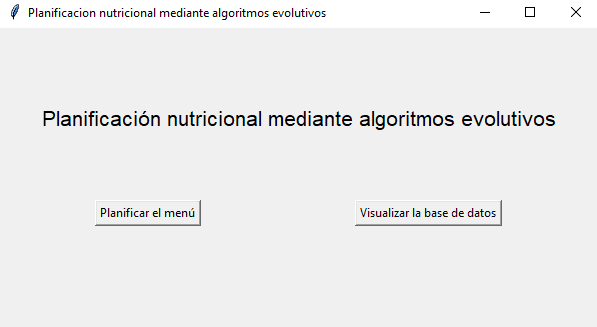
\includegraphics[width=0.9\textwidth]{figures/ventana-main.png}
    \caption{Ventana principal.}
    \label{fig:ventana-main}
\end{figure}

En la ventana \textit{''Base de datos''}, figura \ref{fig:ventana-basedatos}, se ha creado un \textit{''TreeView''} para la representación de los datos. Es una herramienta que permite visualizar y gestionar datos en una estructura de árbol. En este caso tiene una forma de tabla y muestra una lista completa de alimentos, cada uno con su categoría, sus calorías y sus macronutrientes. Además, asociado a este \textit{''TreeView''}, se ha creado un \textit{scrollbar} vertical para poder navegar entre los numerosos alimentos.

Se ha incluido un botón \textit{''Volver''} que redirige a la ventana principal \textit{''Planificación nutricional mediante algoritmos evolutivos''}.

\begin{figure}[H]
    \centering
    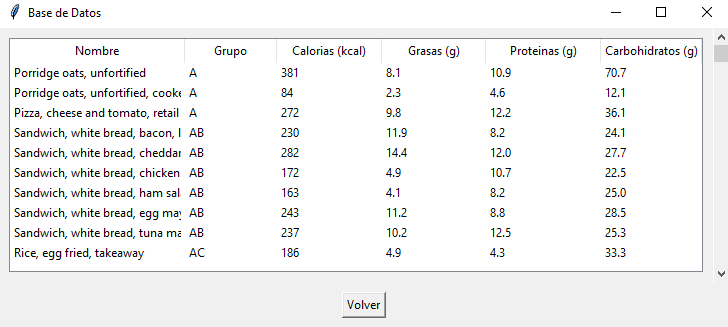
\includegraphics[width=0.9\textwidth]{figures/ventana-basedatos.png}
    \caption{Ventana de la base de datos.}
    \label{fig:ventana-basedatos}
\end{figure}

La ventana \textit{''Preguntas al usuario''}, figura \ref{fig:ventana-usuario}, es usada para calcular las kilocalorías que el usuario necesita y sus grupos alimenticios de preferencia.

Se pregunta al usuario por medio de un \textit{''label''} y este responde en un \textit{''entry''}, que almacena la respuesta. Así ocurre con las preguntas sobre el peso, la edad y la altura. Para el sexo y el nivel de actividad se ha hecho uso de un \textit{''combobox''}, que permite introducir varias opciones posibles dentro de una lista. Para la alergia y las preferencias alimenticias se ha utilizado \textit{''listbox''}, que permite mostrar, correctamente tabulados, todos los grupos de alimentos. Se puede hacer selección múltiple. Estos grupos quedan guardados para luego usarlos durante la ejecución del algoritmo.

El botón \textit{''Calcular calorías''} activa el cálculo de las kilocalorías objetivo del usuario y las muestra. El botón \textit{''Mostrar menú''} activa la ejecución del algoritmo para que encuentre una solución óptima. El último botón, \textit{''Volver''}, regresa a la ventana principal.

\begin{figure}[H]
    \centering
    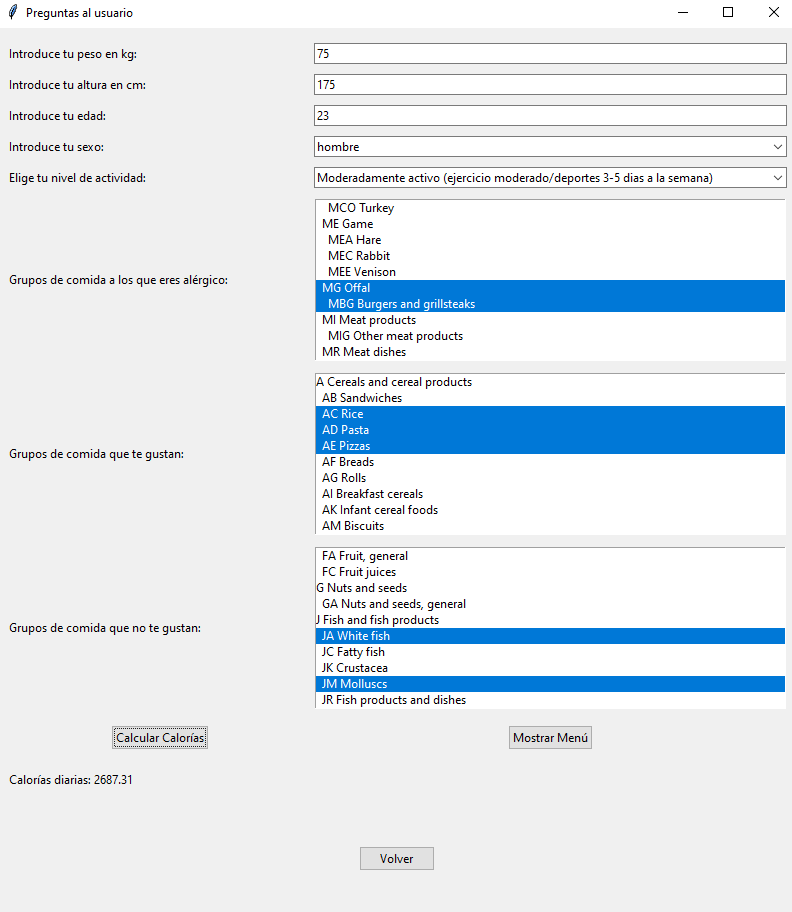
\includegraphics[width=1\textwidth]{figures/ventana-preguntasusuario.png}
    \caption{Ventana de las preguntas al usuario.}
    \label{fig:ventana-usuario}
\end{figure}
\newpage
Tras pulsar el botón \textit{''Mostrar menú''}, el algoritmo se ejecuta con los datos introducidos. Cuando termina, se selecciona la primera de las soluciones no dominadas y se obtiene un menú compuesto por 77 alimentos.

Se ha creado la ventana \textit{''Menú Generado''}, mostrada en la figura \ref{fig:ventana-menu}, donde se ha hecho uso de un \textit{''grid''}, muy útil para la creación de tablas estáticas. Se han introducido 5 filas (comidas diarias) por 7 columnas (días de la semana). Se muestran todos los alimentos que componen la solución elegida, además del grupo al que pertenecen. Se han añadido una fila y una columna como cabeceras, correspondientes a las comidas del día y a los días de la semana, respectivamente. Además, se ha incorporado una fila al final para ayudar a entender si la solución escogida cumple con los objetivos de las kilocalorías y los macronutrientes.

Se han añadido dos botones, \textit{''Atrás''} y \textit{''Cerrar''}. El primero vuelve a la ventana \textit{''Preguntas al usuario''} para la posibilidad de generar otro menú distinto. El segundo botón termina con la ejecución del programa.

\begin{figure}[H]
    \centering
    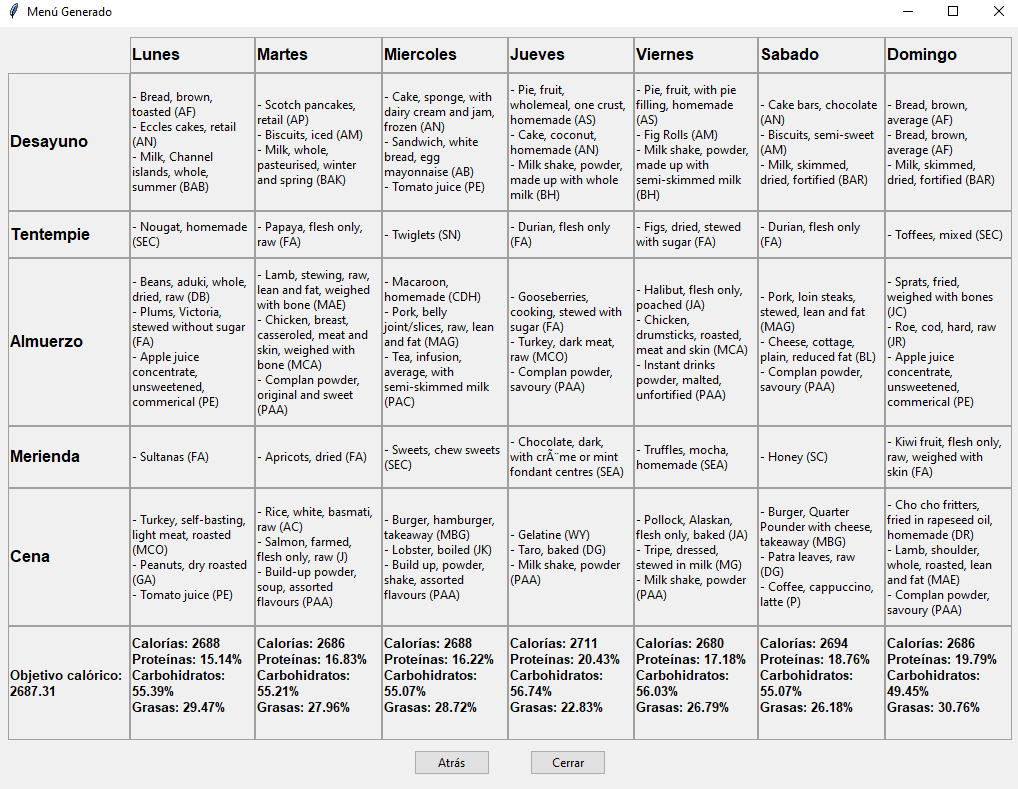
\includegraphics[width=0.965\textwidth]{figures/ventana-menu.png}
    \caption{Ventana del menú generado.}
    \label{fig:ventana-menu}
\end{figure}
\chapter{Configuración de la memoria}

La estructura de esta plantilla está dividida en varios ficheros. Aunque puede parecer complicado, en realidad no es tanto:

\begin{itemize}
    \item \texttt{./appendices/}: Los fuentes de los capítulos de apéndices, vamos, los que van al final y que se usan como adenda a la memoria como tal.
    \item \texttt{./chapters/}: Los fuentes de los capítulos que forman parte del cuerpo de la memoria.
    \item \texttt{./figures/}: Las figuras (imágenes, diagramas) que se usarán a lo largo de todo el documento.
    \item \texttt{./frontmatter/}: Los fuentes de todo aquello que se incluye antes del cuerpo de la memoria. Por ahora, todas las entradas del glosario.
    \item \texttt{./sources}: Ficheros con fuentes que se incluyen dentro de listados de fuentes del documento.
    \item \texttt{./references.bib}: Los fuentes en \hologo{BibTeX} de la bibliografía que se referencia en la memoria en la memoria.
    \item \texttt{./report.tex}: El fichero principal a partir del cual se compila todo el proyecto.
    \item \texttt{./upm-report}: El directorio que tiene todo el contenido que hace que la memoria se vea así. Si tocas aquí, que sea con mimo y cariño, porque es muy fácil cargárselo todo.
\end{itemize}

\section{¿Cómo empiezo a escribir la memoria?}

Por el principio, es decir, con el fichero \texttt{report.tex}. Veamos la primera línea del fichero (listado~\ref{lst:starting-report}).

\lstinputlisting[language=tex,firstline=1,lastline=7,caption=Primeras líneas del fichero \texttt{report.tex},label=lst:starting-report]{report.tex}

En este punto es donde se configura gran parte de la plantilla. Los parámetros y sus opciones son las siguientes:

\begin{itemize}
    \item \texttt{school}: La escuela a la que pertenece el estudiante. La idea de la plantilla es que se use a lo largo de todas las escuelas de la UPM, y que cada una de ellas tenga su propia configuración. La escuela determinará, entre otras cosas, direcciones y colores principales. Las opciones se describen en el~\autoref{ch:escuelas-y-titulos}.
    \item \texttt{type}: El tipo de memoria. Modifica algunos textos, incluida la portada. Puede tomar los valores \texttt{pfg} (\acrlong{pfg}) y \texttt{pfm}  (\acrlong{pfm}).
    \item \texttt{degree}: El grado al que aspira el estudiante. De momento sólo están definidos los grados que se imparten en la ETSISI (también en el~\autoref{ch:escuelas-y-titulos}).
    \item \texttt{authorsex}: Puede ser \texttt{m} (masculino) o \texttt{f} (femenino), y sirve para modificar algunos textos relacionados con el sexo del estudiante.
    \item \texttt{directorsex}: Similar al parámetro \texttt{authorsex}, pero para el director del proyecto.
\end{itemize}

Tras esta configuración, se incluye el fichero de referencias bibliográficas (listado~\ref{lst:starting-references}):

\lstinputlisting[language=tex,firstline=9,lastline=9,caption=Inclusión del fichero de referencias bibliográficas \texttt{references.bib},label=lst:starting-references]{report.tex}

El tema de las referencias bibliográficas se explica en el~\autoref{s:referencias-bibliograficas} del~\autoref{ch:componentes-de-la-plantilla}. En principio no habría que tocar nada (bueno sí, añadir las fuentes y referenciarlas), pero si las referencias se tienen en otro fichero, bastaría con cambiar el nombre al de dicho fichero.

Los cinco siguientes comandos, como se ve en el listado~\ref{lst:starting-title-author-and-director}, indican el título del proyecto, el nombre del autor y su entrada en la bibliografía, y el nombre del director y su entrada en la bibliografía.

\lstinputlisting[language=tex,firstline=11,lastline=15,caption={Configurando autor, título del proyecto y director},label={lst:starting-title-author-and-director}]{report.tex}

El único misterio es eso de las entradas bibliográficas para el autor y el director. No es más que los nombres que aparecen más adelante cuando se indica \enquote{cómo citar el proyecto}. El día que aprenda cómo hacerlo automáticamente, será una configuración que desaparezca\footnote{Bueno, y si tú, queridísimo lector o lectora sabes cómo hacerlo, hazme un \textit{pull request} al repositorio de la plantilla: \href{\templaterepository}{\templaterepository}.}.

Tras ello, empieza el primer contenido de verdad: \textbf{resumen} y \textbf{abstract}, cada uno con sus palabras clave asociadas. Ambos dos son obligatorios y se añaden con la macro \lstinline{\abstract}, donde se especificarán el idioma (\texttt{spanish} o \texttt{english}) y el contenido. De la misma manera, las palabras clave se añaden con la macro \lstinline{\keywords}. Ni que decir tiene que ambos deben tener el mismo contenido, uno en español y el otro en inglés. Y además es obligatorio (según la normativa de la ETSISI).

Existe la opción de añadir agradecimientos a través de la macro \lstinline{\acknowledgements}. Es opcional, así que si no se pone no se renderiza en el documento final, pero es algo bonito y a las abuelas les encanta aparecer ahí. Y las abuelas son de lo más bonito que existe en este mundo, así que cuidadlas.

Y ahora sí, se empieza con el grueso del documento. Tras incluir el glosario, del que se hablará en la sección~\ref{s:glosario} del~\ref{ch:componentes-de-la-plantilla}, se comenzarán a incluir uno tras otro todos los capítulos de los que se compone nuestra memoria, tal y como se muestra en el listado~\ref{lst:starting-include-chapters}.

\lstinputlisting[language=tex,firstline=39,lastline=50,caption={Cómo se incluyen los capítulos y los apéndices},label={lst:starting-include-chapters}]{report.tex}

La macro \lstinline{\appendix} del medio indica a partir de qué punto se añaden los apéndices. No son obligatorios, ni mucho menos, pero en algunos \glspl{pfg} y \glspl{pfm} se suelen incluir para dar información adicional de contexto que no es el objetivo de la memoria, pero sí interesante para complementar. Por ejemplo, en un \gls{pfm} para el estudio del comportamiento de conductores al volante, uno de los apéndices podría ser cada uno de los formularios que se le ofrecieron para rellenar a cada uno de los conductores de dicho estudio.

Y ya estaría todo. Resumiendo, hay que configurar la plantilla, poner el autor, título y director del proyecto e incluir los capítulos y apéndices que queramos.

\section{¿Cómo estructurar la memoria?}
\label{s:como-estructurar}

La respuesta rápida es \enquote{como buenamente quieras/puedas}. En realidad la estructura de la memoria va a depender del tipo de trabajo desarrollado, pero con carácter general, los trabajos suelen seguir ciertas estructuras.

Un \gls{pfg} es un trabajo cuyo propósito es demostrar que se han llegado a adquirir las competencias asociadas con la titulación cursada. Con esto queremos decir que, a diferencia de otros tipos de trabajo académico, en éste no es necesario realizar aportaciones originales al estado de la cuestión.

Una estructura típica es la siguiente:

\begin{enumerate}
    \item Resumen
    \item Introducción
    \item Estado de la cuestión
    \item Metodología
    \item Resultados y Discusión
    \item Conclusiones
    \item Apéndices
    \item Referencias bibliográficas
    \item Glosario
\end{enumerate}

Un \gls{pfm}, a diferencia de un \gls{pfg} trata de profundizar más en un campo concreto de una disciplina, por lo que tiene a ser más extenso y mucho más específico.

En términos generales, la estructura es similar. Sin embargo es de esperar que el nivel de exigencia sea mayor, ya que el estudiante que lo realiza debe demostrar que es un titulado superior. Esto se nota más en la fase de documentación, ya que al tratar de profundizar en un tema más específico, el trabajo de contextualizar y argumentar es más tedioso.

Se pueden identificar dos tipos de proyectos diferentes, aquellos que podríamos catalogar de \textit{profesionales}, con enfoque a la innovación o mejora en un área profesional concreta, y aquellos \textit{de investigación}, más enfocados a la búsqueda de nuevo conocimiento en el área, y que suelen ser el comienzo de la carrera investigadora.

\chapter{Componentes de la plantilla}
\label{ch:componentes-de-la-plantilla}

En este capítulo hablaremos de los componentes principales con los que trabajaremos en nuestra memoria.

\section{Columnas}

TBD

\section{Ecuaciones}

La facilidad de composición de ecuaciones es una de las cosas que más atrae de \LaTeX\space a muchos autores. \LaTeX mantiene dos renderizadores diferentes, uno para el texto y otro para las ecuaciones, denominados modo párrafo y modo matemático\footnote{Existe un tercer modo, denominado \textit{LR mode} o \textit{left-to-right mode}, raramente utilizado y que no trataremos aquí}. El modo párrafo es el modo por defecto y no se le llama explícitamente. Al modo matemático, sin embargo, se le invoca de varias maneras diferentes.

\subsection{Modo en párrafo}

La forma más común es la forma ``en línea'', donde el texto para el modo matemático se encierra entre dos signos \$. Por ejemplo, veamos la frase del listado~\ref{lst:in-line-equation}.

\begin{lstlisting}[language=tex,caption=Ejemplo de inserción de fórmulas en linea,label=lst:in-line-equation]
El pequeño teorema de Fermat dice que si $p$ es un número primo, entonces, para cada número natural $a$, con $a>0$, $a^p \equiv a (\mod p)$
\end{lstlisting}

La frase quedaría como sigue:

El pequeño teorema de Fermat dice que si $p$ es un número primo, entonces, para cada número natural $a$, con $a>0$, $a^p \equiv a (mod p)$

\subsection{Ecuaciones en bloque}

Cuando en lugar de poner una ecuación dentro de un párrafo existente la queremos insertar en su propio espacio independiente hacemos uso de los entorno \texttt{equation} o \texttt{align}, dependiendo de si queremos una o más ecuaciones en el bloque, respectivamente. Por ejemplo, en el caso de una única ecuación, sería similar al ejemplo siguiente:

\begin{minipage}[c]{.5\textwidth}
\begin{lstlisting}[language=tex]
\begin{equation}
	\int_a^b f'(x) \, dx=f(b)-f(a)
\end{equation}
\end{lstlisting}
\end{minipage}%
\begin{minipage}[c]{.5\textwidth}
\begin{equation}
    \int_a^b f'(x) \, dx=f(b)-f(a)
\end{equation}
\end{minipage}

Sin embargo, en el caso de que quisiésemos más de una ecuación en el mismo bloque haríamos uso del carácter \& para indicar en qué punto se alinean las ecuaciones; por ejemplo:

\begin{minipage}[t]{.5\textwidth}
\begin{lstlisting}[language=tex]
\begin{align}
    u  &= \arctan x \\ 
    du &= \frac{1}{1 + x^2}dx
\end{align}
\end{lstlisting}
\end{minipage}%
\begin{minipage}[h]{.5\textwidth}
\begin{align}
    u  &= \arctan x \\ 
    du &= \frac{1}{1 + x^2}dx
\end{align}
\end{minipage}

Por último, si no tenemos por qué referenciarlas en el texto, podemos hacer uso de los entornos \texttt{equation*} y \texttt{align*}

\begin{minipage}[c]{.5\textwidth}
\begin{lstlisting}[language=tex]
\begin{equation*}
	\int_a^b f'(x) \, dx=f(b)-f(a)
\end{equation*}
\end{lstlisting}
\end{minipage}%
\begin{minipage}[c]{.5\textwidth}
\begin{equation*}
	\int_a^b f'(x) \, dx=f(b)-f(a)
\end{equation*}
\end{minipage}

\section{Elementos flotantes}

Vamos a hablar un poco de los elementos denominados \enquote{flotantes} o \textit{floats}. Éstos son bloques de contenido que \enquote{flotan} por la página hasta que \hologo{LaTeX} los coloca donde considera a través de ciertos algoritmos.

Lo general es \textbf{declarar el elemento flotante inmediatamente después del párrafo donde se ha referenciado} (las referencias cruzadas las vemos en la~\autoref{s:crossref} de este capítulo), y después dejar que \LaTeX\space elija el mejor sitio. Y si después de haber escrito todo el documento hay algo que no cuadre, pues ahí modificarlo.

\enquote{¿Y si no hago referencia a un elemento flotante, dónde lo pongo?} Bueno, pues en general no se pone. Si algo no es nombrado, suele ser porque no aporta información, y si no la aporta, pues para qué lo vamos a meter. Ojo, que lo mismo existe algún caso donde sí tiene sentido, pero es muy raro.

Aunque más adelante veremos los diferentes tipos de \textit{floats}, en caso de que queramos modificar su comportamiento todos tienen los especificadores de posición indicados en la tabla~\ref{tab:floats-options}:

\begin{table}
    \caption{\label{tab:floats-options}Opciones para los elementos flotantes de \hologo{LaTeX}}
    \centering
    \begin{tabularx}{\textwidth}{@{}lX@{}}
        \toprule
        \textbf{Especificador} & \textbf{Acción} \\
        \midrule
        H & Colocar exactamente en el sitio indicado                       \\
        h & Colocar aproximadamente en el sitio indicado                   \\
        t & Colocar al comienzo de la página                               \\
        b & Colocar al final de la página                                  \\
        p & Colocar en una página exclusiva para elementos ``flotantes''   \\
        ! & Forzar las opciones obviando los mecanismos internos de \LaTeX \\
    \bottomrule
    \end{tabularx}
\end{table}

\subsection{Código fuente}

Para la gestión de los listados de código fuente se utiliza el paquete \texttt{listings}. El estilo usado es una modificación\footnote{En realidad la modificación es cambiar el fondo de crema a blanco} de \href{https://ethanschoonover.com/solarized/}{Solarized} desarrollado por Ethan Schoonover.

Existen muchas formas diferentes de incluir listados de código en una memoria. Aquí introducimos los más comunes.

\subsubsection{Código dentro del propio párrafo}

TBD

\subsubsection{Bloques de código}

Insertar código en párrafos no es tan común como insertar bloques enteros. Para ello haremos uso del entorno \texttt{lstlisting}. Por ejemplo:

\lstinputlisting[language=tex, firstline=1, lastline=6]{sources/adding-blocks.tex}

Nos daría el siguiente resultado:

\lstinputlisting[language=python, firstline=2, lastline=5]{sources/adding-blocks.tex}

Una cosa que hay que tener en cuenta es que dentro de un entorno \texttt{lstlisting} se ignoran todos los comandos de \LaTeX\space\footnote{En realidad no todos, y si no mira en estos fuentes cómo hemos metido el fin de bloque \texttt{lstlisting} dentro del propio bloque.} y el texto se imprime tal y como se ha introducido. Esto incluye los tabuladores y espacios de principio de línea.

Al igual que en el código de párrafo, también podemos especificar en qué lenguaje está escrito el código para que se resalten en éste las palabras reservadas. Por ejemplo:

\lstinputlisting[language=tex, firstline=8, lastline=14]{sources/adding-blocks.tex}

Nos daría como resultado el siguiente bloque de código:
 
\lstinputlisting[language=python, firstline=9, lastline=12]{sources/adding-blocks.tex}

\subsubsection{Código directamente desde fichero}

Esta forma es muy común, ya que se usa tanto para hacer referencia al código fuente de la aplicación directamente, como a código separado en ficheros para mantener el tamaño de la memoria manejable.

Suponiendo que tenemos el fichero \texttt{sources/snippets.py}, para incluirlo entero basta con usar el comando \texttt{lstinputlisting}:

\begin{lstlisting}[language=TeX]
\lstinputlisting[language=python]{sources/snippets.py}
\end{lstlisting}

Con este comando conseguiríamos el siguiente resultado:

\lstinputlisting[language=python]{sources/snippets.py}

En caso de que se desease importar sólo parte del fichero, se pueden indicar las filas que delimitan el trozo de código. Por ejemplo:

\begin{lstlisting}[language=TeX]
\lstinputlisting[
    language=python,
    firstline=4,
    lastline=5
]{sources/snippets.py}
\end{lstlisting}

Esto haría que sólo se imprimiesen las filas 4 y 5, correspondientes a la segunda función:

\lstinputlisting[language=python, firstline=4, lastline=5]{sources/snippets.py}

Ambas opciones son opcionales, y los valores por defecto de \texttt{firstline} y \texttt{lastline} serán el principio y el final del fichero respctivamente.

\subsubsection{Etiquetando bloques de código}

Al igual que con el resto de bloques \textit{float} (e.g. figuras o tablas), se pueden\footnote{Pongo \textit{pueden} porque es opcional, pero en realidad se \textbf{deben} poner, porque si no los listados de fuentes quedan horribles, como el de esta plantilla por ejemplo (échale un vistazo si no lo has hecho antes).} (\textbf{deben}) añadir pies de texto a los bloques de código, lo cual hace más legible su cometido.

Para ello basta con añadir el argumento \texttt{caption} a las opciones del bloque. Por ejemplo:

\lstinputlisting[language=tex, firstline=15, lastline=20]{sources/adding-blocks.tex}

Nos daría como resultado el siguiente bloque de código:
 
\lstinputlisting[language=python, firstline=16, lastline=19, caption=Función para determinar cuando una palabra \texttt{w1} es anagrama de otra palabra \texttt{w2}]{sources/adding-blocks.tex}

\subsection{Figuras}

El código siguiente (listado~\ref{lst:figure-basic-insert}) renderizará una imagen.

\begin{lstlisting}[language=python, caption=Inserción de una figura,label={lst:figure-basic-insert}]
\begin{figure}[H]
    \centering
    
\includegraphics[width=0.25\textwidth]{figures/vault-boy.png}
    \caption{\label{fig:img-vault-boy} Vault Boy approves that}
\end{figure}
\end{lstlisting}

La sintaxis es bastante autoexplicativa. El entorno \texttt{figure} es el que delimita el contenido de la figura. El comando \texttt{centering} determina que se tiene que centrar . Luego, el comando \texttt{caption} determina el pie de imagen, el cual además incluye una etiqueta (comando \texttt{label}) que sirve para referenciar. Por último, se incluye la imagen con el comando \texttt{includegraphics}.

En definitiva, la imagen (figura~\ref{fig:img-vault-boy}) se mostrará con un ancho igual al 25\% del ancho que ocupa el texto, centrada, con un pie de foto y una etiqueta para referenciar.

\begin{figure}[H]
    \centering
    
\includegraphics[width=0.25\textwidth]{figures/vault-boy.png}
    \caption{\label{fig:img-vault-boy} Vault Boy approves that}
\end{figure}

El comando \texttt{includegraphics} puede importar los formatos típicos de imagen, como jpeg, png o pdf. También admite una serie de opciones como rotación, alto, ancho (éste le hemos especificado con \texttt{width}), etcétera. ¡Ojo! Siempre que se pueda, hay que intentar insertar imágenes vectoriales. De esta manera, se mantiene la calidad de la imagen. Si no, puede ocurrir que se pixele y no quede nada bien.

\subsubsection{Subfiguras}

¿Y qué pasa cuando queremos incluir múltiples imágenes dentro de una figura? Bueno, pues aquí hay que usar el entorno \texttt{subfigure}. En el listado~\ref{lst:subfigure-basic-insert} vemos un ejemplo de cómo se manejan.

\begin{lstlisting}[language=python, caption=Inserción de varias subfiguras,label={lst:subfigure-basic-insert}]
\begin{figure}[H]
	\centering
	\begin{subfigure}{.3\textwidth}
		
\includegraphics[width=\linewidth]{figures/vault-boy.png}
		\caption{\label{fig:subfigure-1}Vault Boy 1}
	\end{subfigure}%
	\begin{subfigure}{.3\textwidth}
		
\includegraphics[width=\textwidth]{figures/vault-boy.png}
		\caption{Vault Boy 2}
	\end{subfigure}%
	\begin{subfigure}{.3\textwidth}
		
\includegraphics[width=\textwidth]{figures/vault-boy.png}
		\caption{Vault Boy 3}
	\end{subfigure}
	\caption{\label{fig:subfigures}Todos los Vault Boy}
\end{figure}
\end{lstlisting}

En realidad cada subfigura se trata como una figura normal, pero en relación con el \textit{float} contenedor. Cuando a una subfigura se le especifica un ancho, se le está diciendo al compilador de qué ancho es esa subfigura en concreto (en nuestro caso 0.3 veces el ancho de la línea). Sin embargo, a la imagen se le da un ancho total de \texttt{linewidth}, porque al estar dentro de su espacio de subfigura, el ancho ha cambiado. El resultado es el que se observa en la figura~\ref{fig:subfigures}. Por cierto, también podemos referenciar a los pies de las subfiguras (e.g. Así:~\ref{fig:subfigure-1}).

\begin{figure}[H]
	\centering
	\begin{subfigure}{.3\textwidth}
		
\includegraphics[width=\linewidth]{figures/vault-boy.png}
		\caption{\label{fig:subfigure-1}Vault Boy 1}
	\end{subfigure}%
	\begin{subfigure}{.3\textwidth}
		
\includegraphics[width=\textwidth]{figures/vault-boy.png}
		\caption{Vault Boy 2}
	\end{subfigure}%
	\begin{subfigure}{.3\textwidth}
		
\includegraphics[width=\textwidth]{figures/vault-boy.png}
		\caption{Vault Boy 3}
	\end{subfigure}
	\caption{\label{fig:subfigures}Todos los Vault Boy}
\end{figure}

\subsection{Tablas}

Las tablas (en realidad \enquote{cuadros}) son una forma muy eficaz de presentar información. En los resultados de casi cualquier trabajo existen cuadros de algún tipo para que los datos se comprendan de un único vistazo (o para que al menos sea más fácil identificarlos.

\notebox{
    \textbf{¿Por qué ``cuadro'' en lugar de ``tabla''?}
    
    Tal y como se indica en el \href{http://www.aq.upm.es/Departamentos/Fisica/agmartin/webpublico/latex/FAQ-CervanTeX/FAQ-CervanTeX-6.html}{FAQ de CervanTex}, \textit{table} (inglés) y \textit{tabla} (español) son falsos amigos; el inglés \textit{table} tiene un sentido más general que el español \textit{tabla}, cuyo uso es únicamente para aquellos cuadros dedicados a la disposición de números (e.g. tabla de multiplicar o tabla de logaritmos).
}

Sin embargo, las tablas suelen ser bastante complicadas en \LaTeX, por lo menos para la gente que empieza. Para no escribir demasiado, la respuesta para casi toda maquetación de tabla está en \href{https://www.tablesgenerator.com/}{https://www.tablesgenerator.com/}. En serio, no perdáis el tiempo si no es estrictamente necesario. La maquetáis visualmente, la generáis (con estilo \textit{booktabs}) y a correr.

\section{Enlaces de hipertexto}

TBD

\section{Fórmulas matemáticas}

TBD

\section{Glosario}
\label{s:glosario}

El glosario de una memoria es el lugar donde se encuentran los términos que se usan a lo largo del documento y que se considera que requieren una aclaración. En esta plantilla, en el momento que generemos un término, se creará un capítulo al final de la memoria con el listado de todos aquellos términos definidos.

Para gestionar el glosario se hace uso del paquete \texttt{glossaries} el cual es relativamente complejo de configurar. También su documentación es muy extensa\footnote{Pero aún así es el sitio donde ir a buscar información. El paquete, junto con su documentación está disponible en la dirección \href{https://www.ctan.org/pkg/glossaries}{https://www.ctan.org/pkg/glossaries}.}, así que en esta sección hablaremos únicamente de lo esencial.

\subsection{¿Cuándo y cómo especificar términos?}

La regla general del \enquote{cuándo} es una vez terminada la memoria. En ese punto, seremos conscientes de qué términos son los más interesantes para incluir en el glosario. En ese punto deberemos ir término por termino sustituyéndolo por la entrada del glosario para que el proceso automático se encargue de la indexación y numeración de páginas.

El \enquote{cómo} se refiere a de qué manera escribirlos. La regla general en el castellano (y hasta donde el autor de la plantilla sabe, en cualquier idioma) es de la manera en la que aparecería en medio del texto. Es decir, si la palabra se escribe generalmente en minúscula (e.g.~\textit{El jugador blandía un \gls{hacha-batalla}}) se deberá incluir dentro del glosario en minúscula, mientras que si se escribe generalmente en mayúscula (e.g.~\textit{Encontró el \gls{arco-perdicion}}) irá en mayúscula.

\subsection{Definiendo los términos del glosario}

Las entradas se escribirán dentro del fichero \texttt{frontmatter/glossary.tex}. La forma estándar de definir un término es la que se muestra en el listado~\ref{lst:std-glossary-entry}.

\begin{lstlisting}[language={[latex]TeX},caption=Código para crear una entrada en el glosario,label=lst:std-glossary-entry]
\newglossaryentry{hacha-batalla}{
    name={hacha de batalla},
    description={Herramienta antigua utilizada en combate}
}
\end{lstlisting}

Luego, dentro del texto, podremos hacer referencia a dichas entradas con los comandos que se muestran en la tabla~\ref{tab:glossary-commands}.

\begin{table}[h]
    \caption{\label{tab:glossary-commands}Comandos para incluir términos del glosario en el texto de la memoria}
    \begin{tabularx}{\textwidth}{@{}lX@{}}
        \toprule
        \textbf{Comando} & \textbf{Ejemplo con la clave \texttt{hacha-batalla}} \\
        \midrule
        \texttt{\textbackslash gls} & \gls{hacha-batalla} \\
        \texttt{\textbackslash Gls} & \Gls{hacha-batalla} \\
        \texttt{\textbackslash glspl} & \glspl{hacha-batalla} \\
        \texttt{\textbackslash Glslp} & \Glspl{hacha-batalla} \\
        \bottomrule
    \end{tabularx}
\end{table}

Como los plurales los gestiona automáticamente, puede ser que queramos, como en este caso, modificar el plural de nuestro término. Para ello debemos añadir la opción \texttt{plural} a la entrada para especificar cómo es el plural de la entrada, como se muestra en el listado~\ref{lst:gls-longplural}.

\begin{lstlisting}[language={[latex]TeX},caption=Especificando el plural para un término del glosario,label=lst:gls-longplural]
\newglossaryentry{python}{
    name={Python},
    plural={Pythonacos},
    description={El mejor lenguaje de programación}
}
\end{lstlisting}

Así, el plural de la clave \texttt{python} descrita quedaría como \glspl{python}, en lugar del valor por defecto que sería \textit{Pythons}.

Un caso particular de términos del glosario son las siglas y los acrónimos. No vamos a entrar en detalle aquí\footnote{Pero recomendamos visitar \href{https://www.fundeu.es/recomendacion/siglas-y-acronimos-claves-de-redaccion/}{https://www.fundeu.es/recomendacion/siglas-y-acronimos-claves-de-redaccion/} y darle una leída porque es interesante.} sino que vamos a introducir las siglas como caso especial de entrada de glosario. Cuando tengamos una sigla, la crearemos en el glosario como se muestra en el listado~\ref{lst:new-acronym}.

\begin{lstlisting}[language={[latex]TeX},caption=Entrada genérica de una sigla o acrónimo en el glosario,label=lst:new-acronym]
\newacronym[
    description={Proyecto Fin de Grado. Proyecto a realizar al final de una titulación de Grado},
    longplural={Proyectos Fin de Grado}
    ]{pfg}{PFG}{Proyecto Fin de Grado}
\end{lstlisting}

En el ejemplo se puede ver que hay dos entradas, \texttt{longplural} y \texttt{description} que son opcionales. La primera es la equivalente a \texttt{plural} de \texttt{newglossaryentry}, y no necesita más explicación.

La segunda, \texttt{description} suele utilizarse para acrónimos, cuando necesitamos describir la entrada. Cuidado en este caso porque si hace referencia a varias palabras estas se deberían incluir dentro de la descripción (como en el ejemplo, \enquote{\acrlong{pfg}}).

La regla general de los acrónimos y las siglas es que la primera vez que aparecen en el texto, deben aparecer con el nombre completo mientras que el resto de veces pueden aparecer indistintamente como sigla o forma larga. De esto se encarga automáticamente el comando \texttt{gls}. Es decir, si tenemos la sigla \texttt{special}, la primera vez que incluyamos la sigla con \texttt{\textbackslash gls\{special\}} saldrá \gls{special} mientras que el resto de veces que la incluyamos se verá simplemente \gls{special}.

Con los acrónimos se incluyen comandos adicionales para controlar su presentación. Estos son los mostrados en la tabla~\ref{tab:acronym-commands}

\begin{table}[h]
    \caption{\label{tab:acronym-commands}Comandos específicos para controlar la presentación de acrónimos}
    \begin{tabularx}{\textwidth}{@{}lX@{}}
        \toprule
        \textbf{Comando} & \textbf{Ejemplo con la clave \texttt{rpg}} \\
        \midrule
        \texttt{\textbackslash acrshort} & \acrshort{rpg} \\
        \texttt{\textbackslash acrshortpl} & \acrshortpl{rpg} \\
        \texttt{\textbackslash acrlong} & \acrlong{rpg} \\
        \texttt{\textbackslash Acrlong} & \Acrlong{rpg} \\
        \texttt{\textbackslash acrlongpl} & \acrlongpl{rpg} \\
        \texttt{\textbackslash Acrlongpl} & \Acrlongpl{rpg} \\
        \texttt{\textbackslash acrfull} & \acrfull{rpg} \\
        \texttt{\textbackslash Acrfull} & \Acrfull{rpg} \\
        \texttt{\textbackslash acrfullpl} & \acrfullpl{rpg} \\
        \texttt{\textbackslash Acrfullpl} & \Acrfullpl{rpg} \\
        \bottomrule
    \end{tabularx}
\end{table}

Por cierto, en castellano las siglas \textbf{no incluyen la \enquote{s} al final}, así que no deberíamos usar los comandos que terminan en \texttt{pl}. Por eso la definición que se ha hecho de la sigla \texttt{rpg} es la mostrada en la figura~\ref{fig:acronym-rpg}.

\begin{lstlisting}[language={[latex]TeX},caption=Entrada de \texttt{rpg} en \texttt{glossaries.tex},label=fig:acronym-rpg]
\newacronym[
    description={Role-Playing Game. Juego de rol},
    shortplural={RPG}
    ]{rpg}{RPG}{\textit{Role-Playing Game}}
\end{lstlisting}

\section{Notas}

TBD

\section{Referencias cruzadas}
\label{s:crossref}

Las etiquetas (\textit{label}) son una herramienta muy útil en el proceso de composición tipográfica. Se puede pensar en ellas como punteros a zonas de interés del documento, de tal manera que se les pueda referenciar sin necesidad de conocer su posición final en la composición.

Por ejemplo, lo normal es que en un libro, a la hora de referenciar una figura, aparezca una frase del estilo ``[\ldots] como muestra la Figura 3 [\ldots]''. Lo que es bastante raro son las frases del estilo ``[\ldots] como muestra la Figura de los moñecos amarillos [\ldots]'' o ``[\ldots] como muestra la siguiente Figura [\ldots]''\footnote{Sí, bueno, quizá la segunda frase no es tan rara, pero siempre es preferible referenciar directamente a dar posiciones relativas.}.

Una de las propiedades más útiles y, en ocasiones, infravaloradas de \LaTeX es la facilidad y potencia de su sistema de etiquetado. Este sistema permite referenciar tablas, listados de código fuente, ecuaciones, capítulos, secciones, etc., con facilidad y flexibilidad. Además, \LaTeX las numera y referencia automáticamente, cambiando la numeración en función de las adiciones y supresiones sin que el autor tenga que hacer nada.

Para referenciar un elemento, lo primero que hay que crear es una etiqueta \textbf{después} del elemento a referenciar. Esto ya lo hemos visto anteriormente, por ejemplo en el listado~\ref{lst:figure-basic-insert}. Si nos fijamos, se declara una etiqueta justo después de la etiqueta \texttt{caption} con el nombre \texttt{fig:img-vault-boy}. De esta manera, podemos referenciar varios indicadores de la figura, como se muestra en el listado~\ref{lst:basic-references}

\begin{lstlisting}[language=tex, caption=Referenciando una figura y su página,label={lst:basic-references},]
Mira la Figura~\ref{fig:img-vault-boy} en la página~\nameref{fig:img-vault-boy}.
\end{lstlisting}

Dicho listado daría el siguiente resultado:

\blockquote{Mira la Figura~\ref{fig:img-vault-boy} titulada \nameref{fig:img-vault-boy} en la página~\pageref{fig:img-vault-boy}.}

\notebox{
    \textbf{¿Por qué a mí me aparece el símbolo \texttt{??} en lugar de una referencia?} Pues lo más seguro es que sea un error a la hora de escribir la etiqueta. Menos común, pero también puede pasar, es que el documento no se haya compilado bien. Hay que tener en cuenta que \LaTeX\space fue creado en una época donde las máquinas tenían poca (¡poquísima!) RAM, y para funcionar lo que se hacían eran varias compilaciones sobre el documento, almacenando los valores temporales en ficheros. Y como nadie quiere perder tiempo en cambiar y \textit{debuggear} algo que funciona estupendamente bien, no se reimplementa. De todas formas, si te animas, ahí tienes un buen proyecto que si lo sacas adelante te va a hacer muy famoso.
}

\section{Referencias bibliográficas}
\label{s:referencias-bibliograficas}

Hay muchas formas diferentes de gestionar las referencias bibliográficas, así que aquí hemos decidido elegir una de ellas por considerarla la más cómoda y simple, que es mediante el paquete \textit{biblatex}.

El fichero de referencias, \texttt{references.bib}, incluirá una entrada por cada una de las referencias que se citan durante la memoria. Luego, en el cuerpo del texto, se podrán hacer referencias a dichas entradas y será \LaTeX~después quien se encargue de indexar correctamente, crear los hipervínculos y maquetar automáticamente.

El fichero \texttt{references.bib} puede tener muchas más de las referencias que se citan en el cuerpo del texto. Sin embargo, sólo aparecerán las referencias que se citen en el texto.

\notebox{\textbf{No has dicho en ningún momento \textit{bibliografía}} Sí. Las referencias bibliográficas, también conocidas como lista de referencias o simplemente referencias, son todas aquellas fuentes bibliográficas que han sido citadas a lo largo del documento. La bibliografía, también conocida como referencias externas, es simplemente una lista de recursos utilizados, citados o no. Como generalmente los no referenciados no se usan para dar soporte a un texto científico se suelen descartar.}
 
\subsection{¿Cómo creamos nuevas referencias?}

El fichero \texttt{references.bib} contará cero o más entradas con la estructura mostrada en el listado~\ref{lst:base-bibref}.

\begin{lstlisting}[language=tex,caption=Estructura general de una referencia,label=lst:base-bibref]
@tipo{id,
    author = "Autor",
    title = "Título de la referencia (libro, artículo, enlace, ...)",
    campo1 = "valor",
    campo2 = "valor",
    \ldots
}
\end{lstlisting}

En esta entrada, \texttt{@tipo} indica el tipo de elemento (p. ej. \texttt{@article} para artículos o \texttt{@book} para libros) e \texttt{id} es un identificador \textbf{único en todo el documento} para el elemento. El resto de campos dependerán del tipo de la referencia, aunque generalmente casi todos los tipos comparten los campos de \texttt{author}, \texttt{title} o \texttt{year}.

\subsection{¿De qué manera puedo citar las referencias?}

TBD~\cite{mcculloch1943logical}

\section{Referencias cruzadas}

TBD

\section{Referencias a recursos externos}

TBD

\chapter{Licencia}
\label{ch:licencia}

Cuando se publica la obra en el archivo digital, por defecto lo hace con la licencia de \textit{Creative Commons} Reconocimiento - Sin obra derivada - No comercial. Aunque usar esta licencia es correcto, no es una licencia libre y a algunos nos parece algo malo.

Considero que todo el conocimiento generado en una universidad pública ha de ser público y libre. Por ello esta obra se publica con la licencia \textit{Creative Commons} Reconocimiento - Sin obra derivada - No comercial - Compartir igual, de tal manera que se garantiza que la obra se comparte con las mismas libertades y así, todo el mundo puede hacer de esta obra el uso que quiera.

\appendix

\chapter{Escuelas y títulos}
\label{ch:escuelas-y-titulos}

A continuación se describen todas las opciones de grados y títulos disponibles en la memoria.

\section{Escuelas}

Las escuelas disponibles se describen en el cuadro~\ref{tbl:schools}.

\begin{table}[h]
    \centering
    \begin{tabularx}{\textwidth}{@{}lX@{}}
        \toprule
        \textbf{Clave}  & \textbf{Valor} \\
        \midrule
        %\texttt{etsii}  & E.T.S. de Ingenieros Industriales \\
        \texttt{etsidi} & E.T.S. de Ingeniería y Diseño Industrial \\
        \texttt{etsisi} & E.T.S. de Ingeniería de Sistemas Informáticos \\
        \bottomrule
    \end{tabularx}
    \caption{\label{tbl:schools} Relación entre el código de la plantilla y la escuela a la que se refiere}
\end{table}

De momento no están todas, así que si te apetece añadir la tuya puedes, o bien contactar con los autores, o bien modificarlo (mira el apéndice~\ref{ch:ampliar}) y también contactar con los autores, así lo podemos hacer público con la mayor cantidad de usuarios posible.

\section{Titulaciones}

Cada una de las escuelas poseen ciertas titulaciones que se han de añadir a la configuración.

\subsection{E.T.S. de Ingeniería y Diseño Industrial}

La ETSIDI tiene configurados como colores principal y de link el RGB $(223,30,64)$. El logo es el mostrado la figura~\ref{fig:logo-etsidi}.

\begin{figure}[h]
    \centering
    
\includegraphics[width=10em]{upm-report/logos/logo-etsidi}
    \caption{\label{fig:logo-etsidi}Logo de la ETSIDI utilizado en la cubierta trasera de la memoria}
\end{figure}

Las titulaciones que existen la última vez que se actualizó este documento son las siguientes:

\begin{itemize}
    \item \texttt{56IE}: Grado en Ingeniería Eléctrica.
    \item \texttt{56IA}: Grado en Ingeniería Electrónica Industrial y Automática.
    \item \texttt{56IM}: Grado en Ingeniería Mecánica.
    \item \texttt{56IQ}: Grado en Grado en Ingeniería Química.
    \item \texttt{56DD}: Grado en Ingeniería en Diseño Industrial y Desarrollo de Producto.
\end{itemize}

\subsection{E.T.S. de Ingeniería de Sistemas Informáticos}

La ETSISI tiene configurados como colores principal y de link el RGB $(0,177,230)$. El logo es el mostrado la figura~\ref{fig:logo-etsisi}.

\begin{figure}[h]
    \centering
    
\includegraphics[width=10em]{upm-report/logos/logo-etsisi}
    \caption{\label{fig:logo-etsisi}Logo de la ETSISI utilizado en la cubierta trasera de la memoria}
\end{figure}

Las titulaciones que existen la última vez que se actualizó este documento son las siguientes:

\begin{itemize}
    \item \texttt{61CD}: Grado en Ciencia de Datos e Inteligencia Artificial.
    \item \texttt{61CI}: Grado en Ingeniería de Computadores.
    \item \texttt{61IW}: Grado en Ingeniería del Software.
    \item \texttt{61SI}: Grado en Sistemas de Información.
    \item \texttt{61TI}: Grado en Tecnologías para la Sociedad de la Información.
\end{itemize}

\chapter{¿Cómo ampliar la plantilla?}
\label{ch:ampliar}

TBD
\chapter{Lista de paquetes incluidos}
\label{ch:paquetes}

TBD

\end{document}
